\documentclass[11pt,a4paper]{article}
\usepackage{amsfonts}
\usepackage{amsmath}
\usepackage{array}
\usepackage{float}
\usepackage[utf8]{inputenc}
\usepackage[czech,english]{babel}
\usepackage{algorithm}
\usepackage{algpseudocode}
\usepackage{xcolor}
\usepackage{textcomp}
\usepackage{todonotes}
\usepackage{hyperref}
\usepackage[final]{pdfpages}
\hypersetup{
	  linktocpage = true,
	  linkbordercolor = yellow
}
\usepackage{tikz}
\usetikzlibrary{trees}
\usepackage{multirow}
\DeclareMathOperator{\EX}{\mathbb{E}}
\algnewcommand\algorithmicforeach{\textbf{for each}}
\algdef{S}[FOR]{ForEach}[1]{\algorithmicforeach\ #1\ \algorithmicdo}

\newenvironment{abstractpage}
  {\cleardoublepage\thispagestyle{empty}}
  {\newpage}
\renewenvironment{abstract}[1]
  {\bigskip\selectlanguage{#1}%
   \begin{center}\bfseries\abstractname\end{center}}
  {\par\bigskip}

% define the title
\begin{document}
\pagenumbering{gobble}

\begin{titlepage}
	\begin{center}
		Czech Technical University in Prague \\
		Faculty of Electrical Engineering \\
		Department of Computer Science \\[1cm]
		
\includegraphics[width=5cm]{figures/lev.pdf}~\\[1.5cm]
		\textsc{\large Master's Thesis}\\[0.5cm]
		
		{\LARGE \bfseries Inventory Optimization Based on Demand Prediction \\[1cm] }

		{\Large Bc. Tomáš Vyskočil \\[1cm]}

		\vfill 
		Supervisor: Ing. Ondřej Vaněk, Ph.D. \\[1cm]
		Study Programme: Open Informatics \\[0.25cm]
		Field of Study: Artificial Intelligence \\[0.25cm]
		May 25, 2018
		
		
	\end{center}
\end{titlepage}

\newpage
\pagenumbering{gobble}
\section*{Acknowledgments}
I would like to thank my supervisor Ing. Ondřej Vaněk, Ph.D. for the advice he has given me, for his patience, and his sense of humor. 


\vfill
\section*{Prohlášení}
Prohlašuji, že jsem předloženou práci vypracoval samostatně a že jsem uvedl veškeré použité informační zdroje v souladu s Metodickým pokynem o dodržování etických principů při přípravě vysokoškolských závěrečných prací. \newline \newline \newline
\noindent
\begin{minipage}[t]{0.4\textwidth}
\begin{flushleft} 
V Praze dne 25.5.2018
\end{flushleft}
\end{minipage}
\begin{minipage}[t]{0.4\textwidth}
\begin{flushright}
Bc. Tomáš Vyskočil
\end{flushright}
\end{minipage}

\newpage
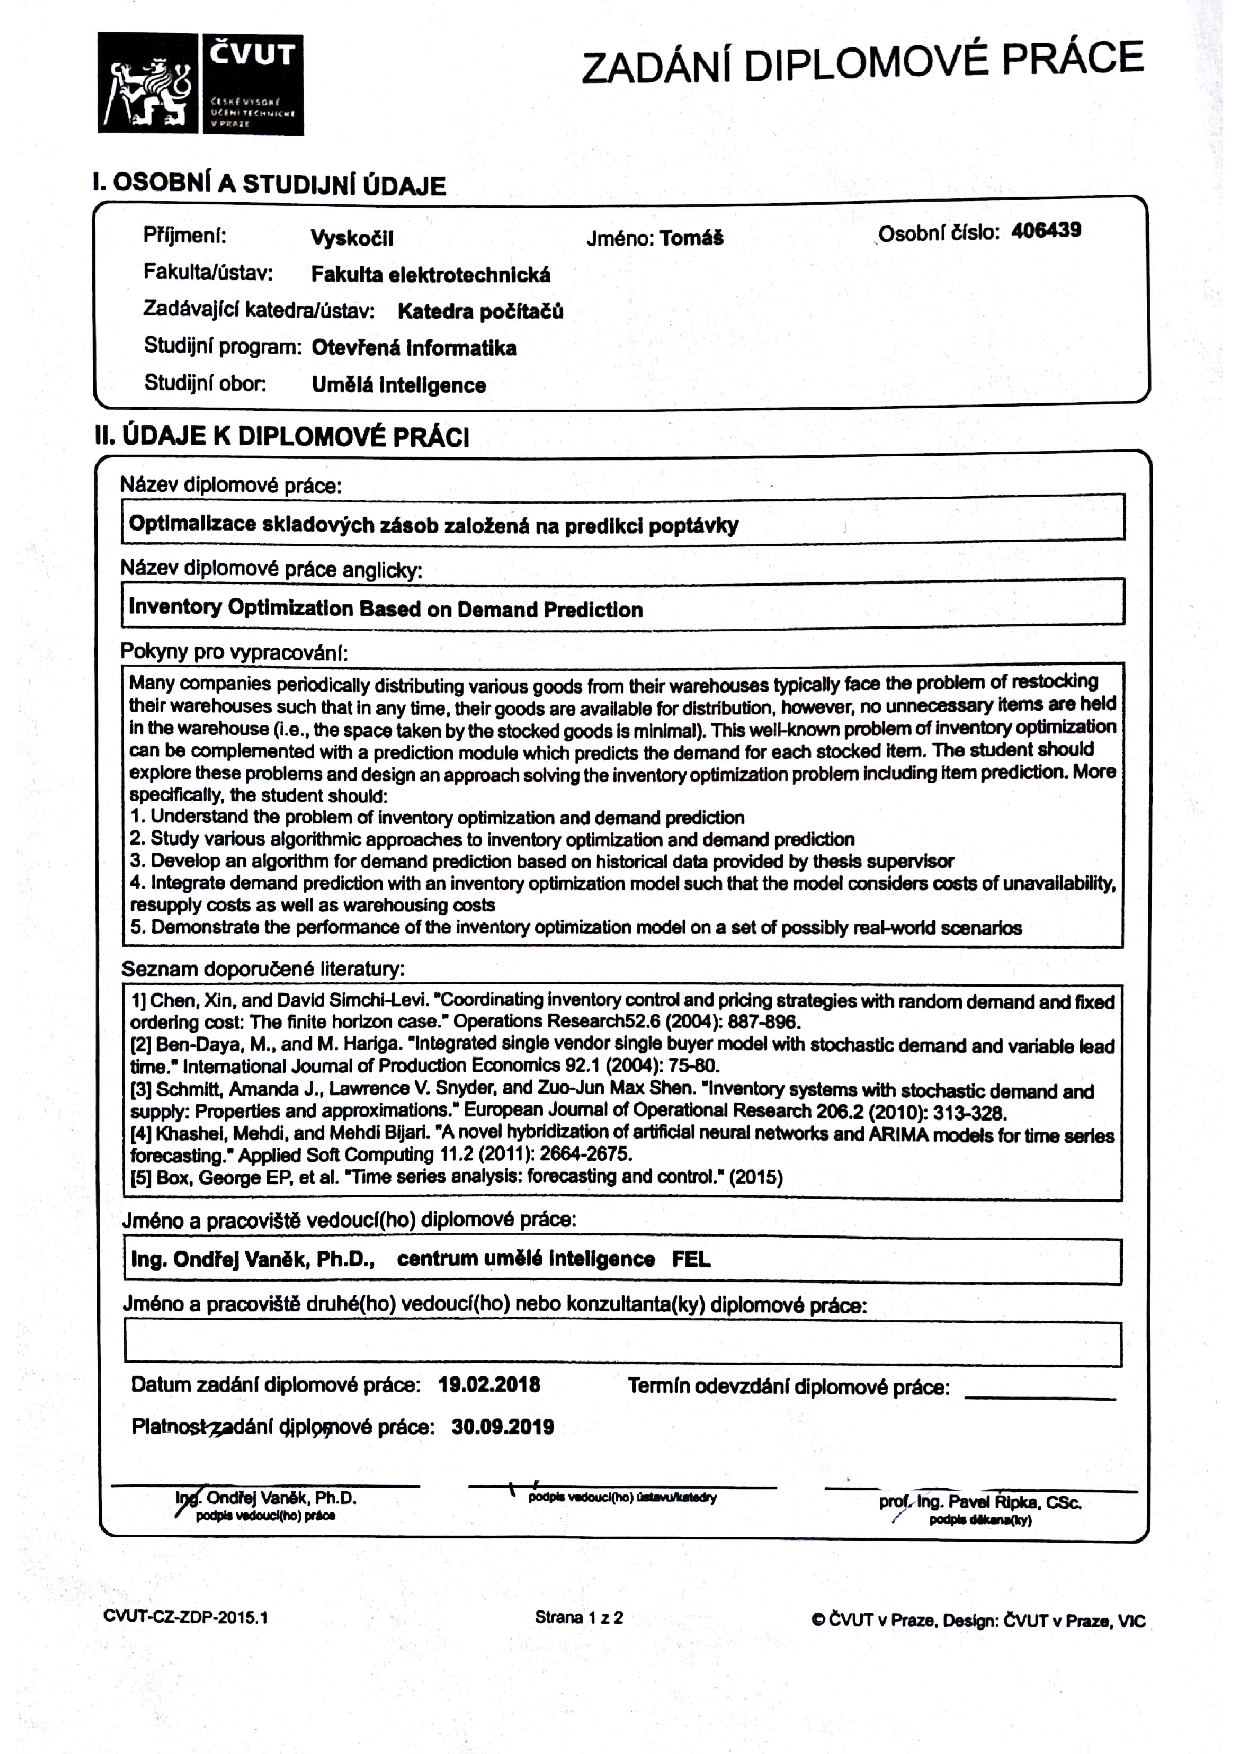
\includepdf{zadani.pdf}
\newpage

\begin{abstractpage}
\begin{abstract}{english}
Efficient inventory management plays an important role for competitiveness of all companies that deliver goods to customers.
The main goal of this thesis is to design an inventory optimization model that makes the best possible ordering policies.

In order to reach this goal, we combine methods of time-series prediction together with stochastic optimization concepts. We create a flexible inventory control pipeline, which is capable of generating goods ordering decisions that consider demand uncertainty, goods durability, shortage costs, warehousing costs, and both fixed and per-unit ordering costs. The pipeline is enriched with the progressive hedging decomposition algorithm, which helps to reduce computation times and improves the capability of our models to reduce risks of unexpected demand outcomes.

\textbf{Keywords:} Time series forecasting, exponential Smoothing, ARIMA, inventory control, stochastic optimization, newsvendor model, decomposition
\end{abstract}

\begin{abstract}{czech}
Efektivní řízení skladových zásob hraje klíčovou roli pro konkurenceschopnost podniků prodávajících zboží.
Hlavním cílem této práce je navrhnout model tvořící objednávky zboží se záměrem optimalizovat vývoj skladových zásob. 

Za účelem dosažení tohoto cíle kombinujeme metody predikce časových řad s koncepty stochastické optimalizace. Práce popisuje tvorbu modulu, který plánuje objednávky s ohledem na neurčitost poptávky, životnost produktů, možné náklady vyplývající z nedostatku zboží, skladováním zboží a objednáváním zboží. Modul je dále vylepšen pomocí „progressive hedging" algoritmu, který snižuje časovou náročnost modulu, a dále vylepšuje jeho schopnost snižovat rizika spojená s neočekávaným vývojem poptávky.

\textbf{Klíčová slova:} Predikce časových řad, exponenciální vyrovnávání, řízení zásob, stochastická optimalizace, newsvendor model, dekompozice
\end{abstract}
\end{abstractpage}

\tableofcontents
\newpage
\pagenumbering{arabic}
\thispagestyle{empty}
\phantom{a} 
\newpage
\setcounter{page}{1}
\section{Introduction}
For many companies, inventory management is one of the most complicated issues in business. Manufacturers, suppliers and retailers need to decide how many goods they need to prevent stock-outs and avoid excess inventory, all this under conditions that can change any time. If they don't meet the customer's demand, the customers can leave for competition. On the other hand, excess inventory can lead to large costs and possible financial loss. This is definition of the inventory control problem, and the solution of this problem should provide a policy in a form that answers question of when and how much goods to order.

Many inventory optimization methods can be used to solve inventory control and other related problems of the companies, depending on the exact conditions in which the company operates. One of the most versatile is the Newsvendor model, which solves the inventory control problem as a trade off between expected leftover and shortage costs, considering stochastic demand.

In this thesis, we propose an extension of the Newsvendor model, which can, based on demand forecast, generate ordering policies for long periods of time. This model can deal with goods durability, fixed and per-unit ordering costs, shortage costs and warehousing costs. All of the costs can be time-dependent. The model also takes the forecast uncertainty into account. Multiple ways of how to tackle the forecast uncertainty exists, but the most promising method is scenario based sampling, which is also used by the model. The finer the sampling, the more precise are the results. Unfortunately, the more samples the model obtains, the higher the computational demands. Therefore we propose a decomposition method for the original model, which solves only an approximation of the original problem, but its computation time grows only linearly with the number of considered demand outcomes. We further evaluate both the original model and the approximating model on real world data, and we discuss the trade off between solving the exact problem with less demand scenarios in consideration, or solving the approximation with much more demand outcomes ``in mind''.

None of the above introduced models could work without a demand forecast, therefore we also study the problem of time series prediction in this thesis.
We develop a demand prediction module, which includes custom extension of exponential smoothing, and the seasonal ARIMA model. We evaluate them both using accuracy measures and visually, and we compare them to another popular forecasting model - the Prophet model. We also examine other properties of the models and their suitability for generation of input to the inventory models.


\newpage
\subsection{Thesis goals}
\begin{enumerate}
\item \textbf{Understand the problem of inventory optimization and demand prediction}

We provide an overview of demand forecasting in \ref{sec:pred_theory} and inventory optimization in chapter \ref{sec:inopt_theory}, we also provide examples of previous related work in chapter \ref{sec:related_work}. Based our findings we develop demand prediction and inventory modules in chapter \ref{sec:approach}.
\item \textbf{Study various algorithmic approaches to inventory optimization and demand prediction}.

We study multiple algorithmic approaches to demand prediction in chapter \ref{sec:pred_theory} and inventory optimization methods in \ref{sec:inopt_theory}. In chapter \ref{sec:related_work} we also provide overview of demand prediction and inventory optimization methods used in previous research and finally in chapter \ref{sec:approach} we use our findings to create a custom solution.

\item \textbf{Develop an algorithm for demand prediction based on historical data provided by thesis supervisor.}

In section \ref{sec:approach_prediction}, we develop an extension of the exponential smoothing algorithm for demand prediction. We also include the seasonal ARIMA prediction model in our demand forecasting module, as it is a proven method for time-series prediction.
We further develop a demand scenario generation module in subsection \ref{sec:approach_scenario}, which generates possible outcomes of the demand according to the forecasts. These demand scenarios are later used as an input to our stochastic inventory models.
\item \textbf{Integrate demand prediction with an inventory optimization model such that the model considers costs of unavailability, resupply cost as well as warehousing costs.}

We develop a custom extension of stochastic Newsvendor inventory model in chapter \ref{sec:sol_inopt}. This model considers costs of unavailability, both fixed and per unit resupply costs and warehousing costs. All of these costs can be time variable and the model considers goods durability as well. We further develop a custom approximation of this model, which can work with more demand information than the base model.

\item \textbf{Demonstrate the performance of the inventory optimization model on a set of possibly real-world scenarios.}

In chapter \ref{sec:eval} we evaluate both the demand forecasting models and the inventory models using real world sales data provided by the supervisor. We first inspect the accuracy and properties of the forecasting models, we also provide a comparison to another popular forecasting approach. In the second half of chapter \ref{sec:eval} we evaluate the inventory models using the real world data. We discuss the trade off between an exact solution with less demand information, and its approximation form which can exploit more information.
\end{enumerate}
\newpage

\section{Technical Background}

\subsection{Time series forecasting}
\label{sec:pred_theory}
Since the target of this thesis is to create an inventory optimization module, which contains a demand forecasting module, we dedicate this section to the field of time series forecasting. Time series is basically anything that is observed over time sequentially \cite{hyndman2014forecasting}, including the demand data that we have at hand.
Time-series forecasting consists of methods which try to predict future values of a sequence based on historical observations. It is a field with many applications, including demand prediction \cite{brown1957exponential}, but also others such as unemployment rate prediction \cite{unempl}.

Before we can create time series forecasts, we need to perform multiple steps. First, we have to gather information about the time series, perhaps historical records, e.g. data including monthly number of airline passengers (the ``Observed" line in figure \ref{fig:passengers}), or other knowledge about the series. Second, we need to perform analysis of the data. This can include search for components like trend - a long term increase or decrease in the series, and seasonality - influence by seasonal factors like week or month or cyclic behavior (long term patterns without fixed period). Examples of both trend and seasonality can be seen in figure \ref{fig:passengers}).
Third, we need to select or create a forecasting model, according to the found properties of the time-series. For example we can select exponential smoothing model or recurrent neural network (examples of other forecasting models are introduced later in this section). After training the model, we can finally create forecasts and evaluate the model using measures like mean absolute error, or we can evaluate the model's performance visually. We can also check the properties (such as normality) of residuals of the model. Residuals of a model are difference between a fitted value and the observed value - can be seen in bottom plot of figure \ref{fig:passengers}. We perform evaluation of forecasting methods in section \ref{sec:dem_eval}. 
\begin{figure}
  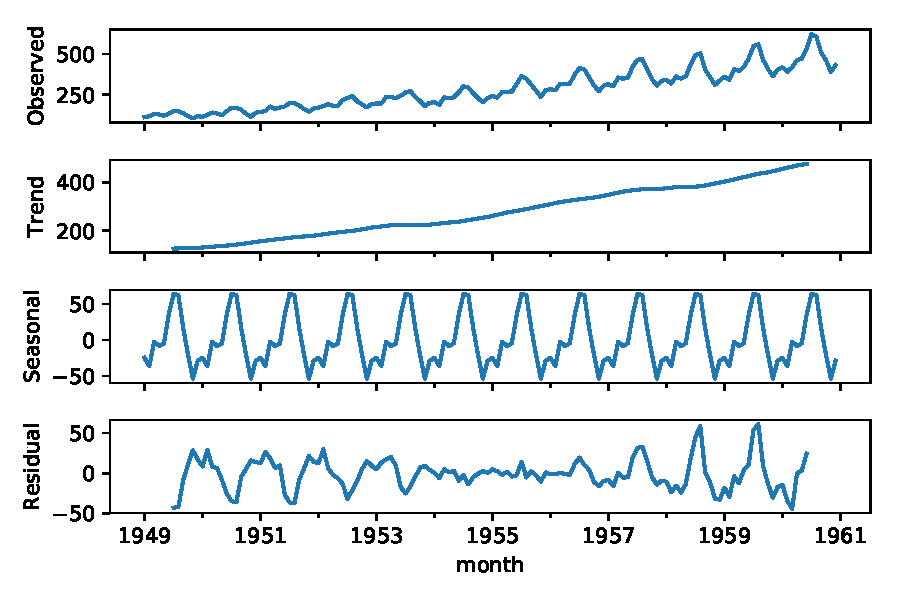
\includegraphics[width=\linewidth]{figures/passengers.pdf}
  \caption{Decomposition of airline passengers time series}
  \label{fig:passengers}
\end{figure}

\subsubsection{Exponential Smoothing}
\label{intro_exp}
Exponential smoothing is a set of methods, which were introduced already in 1950s \cite{brown1957exponential} and have been applied to various problems from many areas such as retail or energy industry. The smoothing methods are still commonly used today, as they enable researchers to quickly create simple and relatively well performing models.  It produces forecasts based on weighted averages of past observations. The name exponential comes from the way this method weighs the past observations, as the weights of older observations decay exponentially, which means that more recent observations are associated with higher weights \cite{hyndman2014forecasting}. 

The simplest of the exponential smoothing methods is called ``simple exponential smoothing''. It provides forecast only based on weighted averages of past observations, but it differs from simple weighted average as the past observations have exponentially decaying weights. We can write the equations for simple exponential smoothing as follows:

\begin{equation}
\begin{gathered}
\begin{aligned}
\hat{y}_{t+1|t} &= l_t \\
l_t &= \alpha y_t + (1-\alpha)l_{t-1}
\end{aligned}
\end{gathered}
\end{equation}
Where $l_t$ is the smoothed value of the series as time t, $y_t$ is the observed value at time t, $\hat{y}_{t+1|t}$ is the forecasted value a time t+1. The parameter $\alpha$ may be selected arbitrarily, or by optimization methods. A common approach is by minimizing some sort of error, most frequently sums of squared errors (SSE), which is defined as follows:

\begin{equation}
SSE = \sum\limits_{t=1}^{T} (y_t - \hat{y}_{t|t-1})^2
\end{equation}
Although the simple exponential smoothing might provide good forecasts in some cases, it is not suitable for forecasting time series with trend or seasonality. To forecast data with trend, simple exponential smoothing was extended to ``double exponential smoothing". The extension consists of adding one more equation to the simple method, which is responsible for smoothing the trend of the series. Double exponential smoothing consists of the following equations:  
\begin{equation}
\begin{gathered}
\begin{aligned}
\hat{y}_{t+h|t} &= l_t + h b_t \\
l_t &= \alpha y_t + (1-\alpha)(l_{t-1} + b_{t-1}) \\
b_t &= \beta(l_t - l_{t-1}) + (1-\beta) b_{t-1}
\end{aligned}
\end{gathered}
\end{equation}
Where $\beta$ is a trend smoothing coefficient, $b_t$ is the trend estimate at time step t and $\hat{y}_{t+h|t}$ is the h steps ahead forecast. 

Even though double exponential smoothing provides a model for wider range of time-series than the simple method, the model does not capture seasonality. Therefore the Holt-Winters method was developed \cite{hyndman2014forecasting}, which adds yet another component to the model - a seasonal component, to improve forecasting of series with seasonality.
Actually two variants of the Holt-Winters method exist, additive and multiplicative.
In this thesis, we use an extension of the additive method, therefore we can show its formulation:

\begin{equation}
\begin{gathered}
\begin{aligned}
\hat{y}_{t+h|t} &= l_t + h b_t + s_{t-m+1+(h-1)mod( m)} \\
l_t &= \alpha (y_t - s_{t-m}) + (1-\alpha)(l_{t-1} + b_{t-1}) \\
b_t &= \beta(l_t - l_{t-1}) + (1-\beta) b_{t-1} \\
s_t &= \gamma(y_t - l_{t-1} - b_{t-1}) + (1-\gamma) s_{t-m}
\end{aligned}
\end{gathered}
\end{equation}
Where $\gamma$ is a smoothing parameter of the the seasonal component, $s_t$, m is the period of the seasonality (e.g. 7 for weekly seasonality and daily data). As in the case of single and double exponential smoothing, the parameters $\alpha$, $\beta$, $\gamma$ can be obtained by minimization. We can see that apart from adding the seasonality term, the level component was adjusted by subtracting the seasonal component.

We should remind the reader, that the are many other possible extensions of exponential smoothing methods, but they are based on the general formulations provided here, a comprehensive list of variants of the exponential smoothing can be seen in \cite{hyndman2014forecasting}. We show some extensions in section \ref{sec:approach_prediction} as we decided to use a variant of exponential smoothing for our demand prediction task.

\subsubsection{ARIMA}
Together with exponential smoothing, ARIMA (Autoregressive Integrated Moving Average) models are the most widely used approaches to time series forecasting \cite{hyndman2014forecasting}.
ARIMA models are a class of models for which some d-th difference of series is stationary \cite{box2015time}. A stationary series is a series whose properties such as mean and variance are not time dependent. For example some series that have a trend or seasonality component are not stationary, but a white noise series is stationary \cite{hyndman2014forecasting}.
An ARIMA model is actually a combination of two models with - the AR (autoregressive) and MA (moving average) model, with \textit{differencing}. Both AR and MA models can be used to model various types of time-series patterns, but they can't be used for non-stationary time-series. 

There are multiple approaches of making a time-series stationary, such as the logarithm transformation, or differencing.
Differencing, which is a process of computing differences of consecutive observations, is used by the ARIMA models.
A differenced series can be written as follows:
\begin{equation}
y_{t}\prime = y_t - y_{t-1}
\end{equation}
Where $y_t$ is the observed value a time t.
Sometimes it is needed to difference the series a second time in order to make it (more) stationary. Second order differencing is defined as follows:
\begin{equation}
y_{t}\prime\prime = y_t\prime - y_{t-1}\prime
\end{equation}
In some cases, seasonal differencing, which is the difference between the current observation and the observation from last seasonality period, is applied:
\begin{equation}
y_{t}\prime = y_t - y_{t-m}\prime
\end{equation}
Where m is the number of seasons. Sometimes it is necessary to do both a seasonal and first order difference to make a series stationary \cite{hyndman2014forecasting}. The order of differencing of ARIMA models is denoted with letter d.

Once we have obtained a stationary series, we can use an autoregressive model of order p - AR(p), which is defined as follows \cite{hyndman2014forecasting}:
\begin{equation}
y_t = c+ \phi_1 y_{t-1} + \phi_2 y_{t-2} + \phi_p y_{t-p} + \epsilon_t
\end{equation}
Where c is a constant and $\epsilon_t$ is an error term. The forecasts of such model are linear combinations of past observations.

We continue with the definition of a moving average model of order q - MA(q), which uses past prediction errors $e_{t-1},\dots,e_{t-q}$ to create a forecast \cite{hyndman2014forecasting}:
\begin{equation}
y_t = c + e_t + \theta_1 e_{t-1} + \theta_2 e_{t-2} + \theta_q e_{t-q}
\end{equation}
By combining differencing of order d, AR(p) model of order p, MA(q) of order q we obtain an ARIMA(p,d,q) model. However ARIMA models are also capable of forecasting seasonal data \cite{hyndman2014forecasting}. By including additional seasonal autoregressive, differencing and moving average terms in the model, we obtain a seasonal $ARIMA(p,d,q)\times(P,D,Q)_m$ (SARIMA) model.
Where:
\begin{itemize}
\item P is the order of the seasonal autoregressive part
\item D is the order of the seasonal differencing
\item Q is the order of the seasonal moving average part
\item m is the seasonality period
\end{itemize}

Further accuracy improvements can be obtained by combining an ARIMA model with a model that considers external factors. In retail industry, such factor could be holidays, price changes or weather. An example of such model is SARIMAX \cite{sarimax}. In general, its forecast can be written as a multi linear regression problem:
\begin{equation}
y_t = \beta_0 +\beta_1 x_{1,t} + \beta_2 x_{2,t} + \beta_k x_{1,k} + \omega_t
\end{equation}
Where $x_{1,t},\dots, x_{1,k}$ are external variables and $\omega_t$ is a residual series, which can be represented as a seasonal ARIMA model.
\subsubsection{Neural networks}
Neural networks are a class methods of artificial intelligence that allow to model complex nonlinear relationships between response variables and predictor \cite{hyndman2014forecasting}. Neural networks also allow forecasting with external factors by just adding another input. This all makes them highly suitable for task of time series prediction. We can name multiple applicable neural network architectures that can be used for the time series forecasting task. From very simple networks that have no hidden layers and only perform linear regression on the data, to feed forward networks, which can use lagged values of the time series to perform auto-regression \cite{hyndman2014forecasting}. Also architectures that contain Long short-term memory (LSTM) units can be used for this task  \cite{laptev2017time} as they have the ability to remember and exploit long term dependencies in data.

\newpage
\subsection{Inventory optimization}
\label{sec:inopt_theory}
In this section we focus on inventory optimization, which is a field of great interest of manufacturers, suppliers, retailers and others.
Inventory optimization aims to create optimal goods (or e.g. materials, components) ordering policies to meet goals such as maximal availability or minimal cost. To meet such goals, inventory optimization tries to answer questions like \textit{what} to order, \textit{when} the order should be placed and \textit{how much} goods should be ordered.
\subsubsection{Costs}
In order to be able answer the \textit{what, when, how much} types of questions, researchers use a wide range of algorithms and models. What many of  these models (and also the approach used in this thesis) have in common, is that for the determination of the inventory policy they work must with at least a subset of the following costs\cite{intro_ls}:
\begin{itemize}
\item \textbf{Procurement costs.} Procurement costs are fixed or variable costs related to acquisition of the goods. These may include per-order fees, per-unit purchase cost, transportation or handling costs.  
\item \textbf{Shortage costs.} Shortage costs \textit{are incurred} when customer demand is not met. This can mean lost sales costs, back order costs or even customer dissatisfaction costs.

\item \textbf{Inventory holding costs.} Inventory holding costs are the costs of storing goods for some period of time. This may include  warehousing costs or \textit{opportunity cost} - the costs for not investing companies capital in more profitable way.

\item \textbf{Obsolescence costs.} Obsolescence costs are the costs of lost value of stocked items. This can mean deteriorating food or flower inventories, clothing items going out of fashion etc. 
\end{itemize}
\subsubsection{Modeling}
As already stated, researches use many types of models to solve inventory optimization problems.
In this thesis, we don't focus on deterministic models such as \textit{Economic ordering Quantity} \cite{eoq}, where demands, prices etc are known, even though they have a broad range of applications. Instead, we mainly focus on the class of \textit{stochastic} models. In the following lines we introduce two such models, the Base Stock \cite{supply} model and the Newsvendor model \cite{sp_book}.

\subsubsection{Base stock model}
The first stochastic inventory model we will introduce is the Base Stock model, which is a well known model that can provide ordering policy for infinite number of periods.
However, the model is in its base form is very limited, as it provides only the ordering amount based on random demand data and expected service level (the probability of not stocking out). It also assumes that products can be analyzed individually and replenishments have known lead time (the time required between making an order and receiving the goods). In addition, only fixed ordering costs are considered by the model.

The steps of the model can be described as follows \cite{supply}:
\begin{itemize}
\item First we need to determine the review period (the time between successive revisions of the inventory) denoted \textit{T}:
\begin{equation}
T = \sqrt[]{\frac{2K}{h\mu}}
\end{equation}
Where K is fixed ordering cost, h is daily holding cost(the cost of keeping one unit of product in inventory) and $\mu$ is mean daily demand.

\item If we assume the demand during review period \textit{T} is from normal distribution with mean $\mu$ and variance $\sigma^2$, the ordering amount S for given service level $\alpha$ according to base stock model is:
\begin{equation}
S_T = \mu + z(\alpha)\mu
\end{equation}

Where $z(\alpha)$ is the value of the inverse cumulative distribution function of standard normal distribution for $\alpha$.
\end{itemize}
The model could be theoretically adjusted, so that it considers more inventory aspects like goods durability - by modifying the review period.
However, it is not suitable at all for optimizing orders according to goods ordering (or other) costs changes. Therefore in the following sections we introduce the Newsvendor model, which has a very flexible linear programming formulation.

\subsubsection{Stochastic programming}

Before we introduce another stochastic inventory model - the Newsvendor model, we should also briefly provide introduction of the area of Stochastic programming, whose concepts are used by the Newsvendor model \cite{sp_book}.


Stochastic programming is an approach for modeling and solving optimization problems that involve uncertain parameters \cite{sp_tut}. Even though there are many other ways how to solve problems involving uncertainty, stochastic programming has proven its usefulness in many areas such as telecommunications, economics, energetics or medicine \cite{sp_book} \cite{hydro} \cite{surgery} \cite{telco}. A common application of stochastic models is in a setting when a decision must be made \cite{sp_book}, for example in problem of investment portfolio optimization. If we knew exactly the future value of the possible investments, we could create a deterministic model that would give us the optimal portfolio. However in real world scenario we usually don’t have such precise information, and we have to work (for example) with probability distribution estimates created from data that have been collected over time (in case of portfolio optimization problem that would be the investment future value probability distribution).

In the following lines we introduce some of the basic terms and methods related to stochastic programming.  We will illustrate them using the stochastic Newsvendor model, which itself serves as a base for solution of the inventory optimization problem introduced by this thesis. 

\subsubsection{Newsvendor (Inventory) model}
\label{sec:nwi}
The basic newsvendor model is another stochastic model used to determine optimal inventory levels. Its goal is maximizing expected profit by finding an optimal trade-off between risk of over-stocking and the risk of under-stocking. In the basic setting, the model assumes zero ordering lead time, no ordering and inventory amount limits and allows inventory shortages. Also the basic setting only provides ordering policy for one ordering period and for one product. However, as the model solution also has linear programming formulation, it can be easily extended. In contrast with the Base Stock model, the model accounts for cost of goods unavailability \cite{supply}.

The output of the model is the ordering quantity x, which should satisfy the demand d. The unit ordering cost is c. If the demand is greater than the ordered amount of units, a per unit backorder penalty b is incurred.  On the other hand, if the demand is smaller than x, a per unit holding cost is incurred. The objective is to minimize the total cost G(x,d), which is defined as follows \cite{sp_tut}:
\begin{equation}
G(x,d)= cx +b\lbrack d - x\rbrack_+ + \lbrack x-d \rbrack_+ 
\end{equation}
Where $\lbrack a \rbrack_+$ denotes the maximum of a and 0. \\
However in the common real world case, the retailer does not know the demand d, as e.g. he needs to determine the optimal inventory level before a sale season with uncertain demand. To cope with this, we can view the demand \textit{D} (denoted by \textit{D} to highlight that we mean the random variable instead of its particular realization \textit{d}) as \textit{random variable} \cite{sp_tut}. If we assume that the distribution of D is known, because we can for example estimate it from past demand observations, we can define the following optimization problem, which aims to minimize total cost expected value \cite{sp_tut}.

\begin{equation}
\underset{x\geq 0}{min} \EX\lbrack{G(x,D)} \rbrack
\end{equation}

The goal of the above mentioned problem is to minimize the total cost \textit{on average}, its justification comes from the Law of Large Numbers \cite{sp_tut}. In case of the basic Newsvendor problem, the expected value formulation has a closed form solution. However, this is not always the case in stochastic programming problems. One way to tackle this is using \textbf{scenarios}. We can illustrate the scenario approach using the Newsvendor problem as well \cite{sp_book}. 

Let's now suppose that the demand random variable D has a finitely supported distribution, which means it takes values $d_{1}$, ..., $d_{k}$, called \textit{scenarios}, with respective probabilities $p_{1}$,..., $p_{k}$. In such case we can model the stochastic program as deterministic optimization problem and write the expected cost as the following sum:

\begin{equation}
 \EX \lbrack G(x,D) \rbrack = \sum\limits_{k=1}^{K}{p_k G(x, d_k)}
\end{equation}

And to obtain the ordering quantity x, that minimizes the expected cost, we can use to solution of the following linear program:

\begin{equation}
\begin{gathered}
\underset{x,t_1...t_k}{min}\quad 
\sum\limits_{k=1}^{K}{p_k t_k} \\
\begin{aligned}
 \textup{s.t.}\quad (c-b)x -t_k & \leq  -b d_k,\ k = 1,...,K  \\
 (c+h)x -t_k & \leq h d_k,\ k = 1,...,K  \\
x & \geq 0
\end{aligned}
\end{gathered}
\end{equation}

Using the concept of scenarios we obtained the ``extensive" form of the problem, which is a tractable approximation of the expected value problem. The scenarios can be obtained in very diverse ways, they can be samples from a known discrete probability distribution, or they can be result of discretization or simulation, the source can of scenarios can also be some limited sample information, and others. This kind of model is also called the a two stage stochastic programming model, as in the first stage we make some decision (orders) that has some cost, and in the second stage we deal with the consequences of the decision and we ``pay" the costs related to the consequences.

So far we have introduced only a relatively limited version of the Newsvendor problem (and stochastic programming problems in general), where only one decision is being made at one point in time. However it is quite common that we want to solve a problem where decisions (e.g. order amount) will be made sequentially at certain periods of time, and each decision should be made using the knowledge of outcomes of previous decisions (e.g. leftover inventory). This type of problems are called \textbf{Multi-stage stochastic} problems. 

In the multistage Newsvendor problem, we suppose that the retailer has a finite planning horizon of T periods, and the demand is modeled as a random process $D_t$ indexed by the time t = 1, ..., T \cite{sp_book} At each stage t = 1, ..., T, the retailer observes the current inventory level $y_t$, and replenishes the inventory to level $x_t$ by ordering $x_t-y_t$ units. Then the starting inventory level at time t+1 $y_{t+1}$ is obtained from equation $y_{t+1} = x_t - d_t$, where $d_t$ is a particular demand realization at time t. The objective is to minimize the expected total cost over the planning horizon, which we can write as follows \cite{sp_book}:

\begin{equation}
\begin{aligned}
\underset{x_t \geq y_t}{min} & \quad
\sum\limits_{t=1}^{T}{\EX \{ c_t (x_t - y_t) +b_t\lbrack D_t - x_t\rbrack_+ + h_t \lbrack x_t-D_t \rbrack_+ \}} \nonumber 
\\
\textup{s.t.} & \quad y_{t+1} = x_t - D_t, \ t = 1,..,T-1  \\
\end{aligned}
\end{equation}

As in the simple (single stage) model, we can again employ the concept of scenarios, or more precisely, \textbf{scenario trees}. If we consider the random process $\xi_1$, ..., $\xi_T$ has a finite number (K) of realizations ($\xi^1,..., \xi^k$), we can depict the possible sequences in a form of a scenario tree (see example in figure \ref{fig:tree}). In general, nodes at each level t of the tree represent all possible values of $\xi^t$. The tree has only one node at level t = \,1, which branches in nodes at level t = 2, the branching continues up to level t =\,T. However the branching factor does not have to be same for all nodes, as the reader can see in the example. Numbers along arcs between nodes represent conditional probabilities of moving to next node.
Each scenario is represented as a path from the root at level t = 1 to some node at the last level t = T. The probability of the scenario can be computed by multiplying the transition probabilities written along the path segments.
As an example we can take scenario $w^s$\,= ($\xi_1^s$, $\xi_2^s$ $\xi_3^s$)\,= (1, 3, 5), which has the probability $p^s = 0.25 \cdot 1$.
\begin{figure}
\begin{tikzpicture}[level distance=1.5cm,
level 1/.style={sibling distance=3.5cm},
level 2/.style={sibling distance=2cm}]
\tikzstyle{every node}=[circle,draw]
    \node (Root) {1}
        child  { 
        node {6}  
        child { node {4} edge from parent node[right,draw=none] {0.3} }
        child [black] { node {5} edge from parent node[right,draw=none] {0.3} }
        child [black] { node {6} edge from parent node[right,draw=none] {0.4} }
        edge from parent node[right,draw=none] {0.5}
    }
    child {
        node {3}
        child { node {5} edge from parent node[right,draw=none] {1}}
        edge from parent node[right,draw=none] {0.25}
    }
    child {
        node {2}
        child { node {4} edge from parent node[right,draw=none] {0.2}}
        child { node {7} edge from parent node[right,draw=none] {0.4} }
        child { node {5} edge from parent node[right,draw=none] {0.4}}
        edge from parent node[right,draw=none] {0.25}
        };
   % Comments to each level
   \begin{scope}[every node/.style={right}]
     \path (Root    -| Root-3-3) ++(5mm,0) node {t = 1};
     \path (Root-1  -| Root-3-3)++(5mm,0) node {t = 2};
     \path (Root-1-1  -| Root-3-3)++(5mm,0) node {t = 3};
   \end{scope}

\end{tikzpicture}
\caption{Scenario tree example}\label{fig:tree}
\end{figure}


Finally, we can write the following linear program, which enables us to find optimal ordering amounts under each scenario and time stage t $x_{k,t}$, where k is the number of scenarios and k is the number of stages.

\begin{equation}
\begin{gathered}
\min_{x_{k,t}} \quad 
\sum\limits_{k=1}^{K}{ p_k \sum\limits_{t=1}^{T}{ z_{k,t} }} \\
\begin{aligned}
\textup{s.t.}\quad  & z_{k,t}  \geq (c_t-b_t)x_{k,t} + b_t d_{k,t} -c_t y_{k,t} ,\ k = 1,\dots,K,\  t = 1,\dots,T\\
                  &z_{k,t}  \geq (c_t+h_t)x_{k,t} - h_t d_{k,t} -c_t y_{k,t} ,\ k = 1,\dots,K,\  t = 1,\dots,T  \\
         & x_{k,t} \geq 0 \\
         & y_{k,t+1}  \geq x_{k,t} - d_{k,t}
\end{aligned}
\end{gathered}
\end{equation}
Where $c_t$, $h_t$, $b_t$ are the per unit ordering, holding and shortage costs at time stage t, $d_{k,t}$ is the demand at time stage t under scenario k, $p_k$ is probability of scenario k, $x_{k,t}$ is the inventory level at time stage t under scenario k, $y_{k,t}$ is leftover inventory from stage t-1 under scenario k, $z_{k,t}$ is expected cost at time stage t under scenario k.


However, such model does not make sense, because it allows different decisions for scenarios with common history, and also allows the decision to be adjusted according to future stochastic realizations. Therefore \textit{non-anticipativity constraints} need to be added to the linear program, ensuring that each decision $x_{k,t}$ depends only on information known up to stage \textit{t} under scenario \textit{k}. The non-anticipativity constraints look as follows \cite{sp_book}:

\begin{eqnarray}
x_t^k = x_t^l,\ \forall{k,l}\ \text{for which } \xi_{\lbrack t \rbrack}^k=\xi_{\lbrack t \rbrack }^l,\ t = 1, \dots,T
\end{eqnarray}

Where  $\xi_{\lbrack t \rbrack}^k$ denotes the scenario history up to time t. For example if $\xi^k  = (2,3,4)$, then its subsequence until t = 2 is  $\xi_{2}^k = (2,3)$.

So far, we have shown how to create a multi stage stochastic linear program. However, with increasing number of stages or scenarios, such linear program can easily become untractable in some way. It can happen that the model does not fit in computer's RAM or it is very computationally demanding. To overcome this, researches can use simple techniques such as limiting the number of scenarios, for example by decreasing the branching factor from some later stage, or by grouping the stages \cite{sp_tut}, e.g. in the case of Newsvendor, weekend days can be grouped with Fridays if orders can't be made during weekend. Researchers can also employ more sophisticated approaches, such as:
\begin{itemize}
\item \textbf{Sample average approximation} \\
This method uses a Monte Carlo simulation to obtain a problem of a manageable size. It approximates the original stochastic expectation function by generating iid samples $\xi^1$, ..., $\xi^N$ of random vector $\xi$, and for this sample it solves the deterministic equivalent problem (the sample is used as a set of scenarios). By sampling and solving the deterministic problem, it obtains a set of candidate solutions, which are later compared by computing the optimality gap \cite{sp_book}.
\item \textbf{Benders decomposition}
Benders decomposition \cite{benders1962partitioning} is one of the decomposition approaches often employed in context of stochastic programming. In general, it decomposes linear programs in a relaxed master problem and subproblems by fixing some of the variables in the linear program. The master and subproblems are being solved iteratively. By solving the subproblems, we obtain feasibility and optimality constraints for the master problem. In multi stage setting, the master problem is always represented by decision at some node of the scenario tree, the subproblems are represented by decisions at its children nodes. 
\item \textbf{Progressive hedging algorithm}
Progressive hedging algorithm (PHA) is another decomposition method often used in context of stochastic programming. It was introduced by Rockafellar et al. \cite{rockafellar1991scenarios}.In contrast with Benders decomposition, it decomposes the original problem by whole scenarios, not by each decision in the scenario tree. We will further introduce this decomposition method in following sections.

\end{itemize}
\newpage
\section{Related work overview}
\label{sec:related_work}
In this chapter we offer a brief overview of related previous work. The chapter is divided in two sections, one covers previous work related to demand and general time series forecasting, the second provides a summary of previous work related to inventory optimization.
\subsection{Time series forecasting}

The field of time series forecasting was strongly influenced by book of Box and Jenkins \cite{box2015time}, where they offer a guide to ARIMA model identification, estimation and verification \cite{de200625}. Popularity of their approach most likely arises from the versatility of the guide along with the ability of ARIMA models to fit various types of data. Hyndman et al. \cite{de200625} provide a list with examples of research papers dedicated to time series forecasting, 9 of them used an ARIMA model, for instance to predict truck sales (in \cite{heuts1988forecasting}) or telecommunications traffic (\cite{layton1986international}). More recently, researchers use ARIMA models as a benchmark model, e.g. in Zhang et al.\cite{zhang1998forecasting}, or they use hybrid approaches of modeling, which combine ARIMA models with other approaches, such as Neural Networks \cite{zhang2003time}. 

Another commonly used forecasting method is exponential smoothing and its extensions. Exponential smoothing, was first introduced under the name in exponential smoothing \cite{brown1957exponential}, where the author used the method for demand forecasting. This exponentially weighted average method was later updated by Holt \cite{holt2004forecasting}, who added a trend component to the model. Later Winter  \cite{winters1960forecasting}, in a research paper dedicated to sales forecasting, updated the model with a seasonality component, and thus created the Holt-Winters forecasting method. The model was further extended by multiple authors, for example with components helping in prediction of time series with multiple seasonalites \cite{shahin2017using}.

In general, researchers apply many other approaches than just extended exponential smoothing models or ARIMA based models. With the massive popularity of deep neural networks in recent years, it is no surprise that researchers have also applied its concepts to time series forecasting. For instance in \cite{zhu2017deep} the authors apply a deep model to taxi demand prediction, or in \cite{orozco2018mordred} they develop a model, which they benchmark on tide height prediction.

\subsection{Inventory optimization}
To our own knowledge, there are no previous works on the topic of multi-period Newsvendor with time-variable costs and deteriorating items, but in general, there are many works solving various other extensions of the Newsvendor  problem.
However, we should mention that not all research work focuses on the case with stochastic demand, even though some studies on the topic of inventory problem with stochastic demand date back to 1958 \cite{scarf1958min}. Other researchers also focus on models which ignore some of the relevant costs.

A lot of research work focuses only on the inventory optimization part of the problem introduced in this thesis, however some works try to solve both the demand forecasting problem and the inventory problem as in this work. For instance Levina et al. \cite{levina2010weak} propose an online algorithm for the Newsvendor problem, which can be used in case no prior demand distribution information is known. Also Oroojlooyjadid et al. \cite{oroojlooyjadid2016applying} provide an end to end solution for the newsvendor problem. They propose a deep neural network based approach, which, using previous demand data and observed features, directly outputs future ordering policy. Ning et al. \cite{ning2009fulfillment} also use neural networks to predict warehouse customers' demands based on which they create ordering policies. Sachs et al. \cite{sachs2015data} focus on Newsvendor problem adjusted for the problem of censored demand. Censored demand occurs in case the demand is greater than the available inventory, as in such case we don't know the exact demand, which can further affect future demand predictions.


After reading the previous paragraphs the reader might think that most solutions of inventory optimization problems revolve around application of mixed integer programming or neural networks. However the range of techniques is wider. As an example we can name Daniel et al.\cite{daniel2005simulation}, which combine a simulation and genetic algorithm approach to optimize a supply chain inventory costs.

We can also name a few authors, that solved a more closely related problem to the optimization part of this thesis, we can start with Kim et al. \cite{kim2015optimal}.
Kim et al. focus solely on the inventory problem and provide solution to multi period Newsvendor problem
with transhipments. They provide an MILP formulation of the problem, which they try to solve more efficiently with the Progressive hedging decomposition method. They work also includes a table with comparison of works of other authors related to topic of (extended) Newsvendor problem.
We can also mention Levi et al., as \cite{levi2007provably} they solve the regular multi period Newsvendor problem by the Simple Average Approximation approach. They also provide formal proofs of how many samples are required to guarantee that the sampling approach solution is close to optimal solution with arbitrary precision.

Finally, we can state that (to our knowledge) none of the previous works proposes a model of retailer that would be suitable for purposes of this work, as our approach provides ordering policies for multiple steps ahead, considers demand uncertainty, fixed ordering costs,
goods durability, disallows back orders (back-order means that part of customer demand from one period can be satisfied in next periods). Also to our knowledge, none of the works suggests to use progressive hedging decomposition approach in order to significantly increase the number of demand scenarios considered by the model.

\newpage
\section{Solution approach}
\label{sec:approach}

\subsection{Motivation}
Inventory control plays an important role for competitiveness of any company that provides goods for its customers. An example of such company could be an online store, which both delivers and distributes groceries. Goods shortages cause lower profits and they can easily lead to customer dissatisfaction. On the other hand excess inventory may force the store to sell goods at lower prices, or even worse it can lead to inventory write offs. Higher inventory levels also increase warehousing costs.

A module that would be able to forecast demand with high accuracy, combined with a precise inventory model, that accounts for possible errors of the forecasting module and considers all inventory related costs and goods durability, would be of great use for such companies. In this thesis we aim to create such module, with the focus on precise modeling of an online grocery store.

\subsection{Assumptions}
During the preparation of the solution approach used in this thesis, we had to make a few assumptions as it helped us to overcome technical difficulties, e.g. in case we did not know some parameters.
The list of the most important assumptions with brief justification follows:
\begin{itemize}
\item Censored demand: Our models don't take censored demand into account. Censored demand occurs when demand is greater than the available stock. In such case, we only know that the demand was greater than the stock level, but we do not know the exact demand. Some research on this topic has been done by other authors  e.g. \cite{sachs2015data}.
\item Product class prediction/ordering: During the initial research phase, we have found it very difficult to predict single product class demand. There are many possible reasons. One reason could be variance in product availability, or product sale discontinuation, e.g. because of new product. Therefore we focus on prediction and generation of inventory policies of \textit{product classes}, instead of single products. This means, for example, that we predict the demand for all bananas, instead of single brand of bananas.
\item Product class policy: Our models currently provide only product class ordering policies instead of per-product policies or whole multi-item policies.
\item Expired products: We assume that expired products are removed immediately after expiration and older products are sold before new products.
\item Zero order lead time (the time between making an order and receiving the order): During the preparation of this thesis we did not have access to length of order lead time so we do not consider it in our models.

\end{itemize}

\subsection{Preprocessing}
During initial research phase we have studied the influence of preprocessing methods on the accuracy of the demand forecasts. First we tried remove outliers from the historical data by smoothing methods, later we also tested the Hampel filter \cite{hampel}, which measures deviation of time series samples from median of their surrounding samples, and removes those samples that differ significantly from the median. However, the best results were obtained by simply replacing values that coincided with non-working holidays, as these samples were unnecessary outliers in the series, which can potentially harm the fitting process of the forecasting models.

\subsection{Demand prediction}
\label{sec:approach_prediction}
Even though the inventory model presented in section \ref{sec:sol_inopt} can account for possible errors of the forecasting module that precedes it, the accuracy of the demand forecasts still plays a crucial role for its performance. Therefore we use the ARIMA and exponential smoothing methods which have many times proven its ability to provide accurate forecasts.
\subsubsection{ARIMA model}
The first model we decided to include is the seasonal ARIMA$(p,d,q)\times(P,D,Q)_m$ as it was many times successfully used for forecasting time-series from various areas. 
Because our inventory pipeline is expected to work automatically, we had to create an automated method of the model order selection. Our approach is based on a grid search approach, which tests various model order configurations. The final model order is selected by minimizing the Bayesian information criterion (BIC) \cite{hyndman2014forecasting}:

\begin{equation}
BIC = AIC + (log(T) -2)(p+q+k+1)
\end{equation}
Where AIC is the Akaike information criterion, which is defined as follows:
\begin{equation}
-2log(L) + 2(p+q+k+1)
\end{equation}
and L is the value of maximum likelihood function of the model, k is the number of parameters of the model, p is the autoregressive order and q is the moving average order of the model, T is number of observed samples.

To narrow down the number tested model configurations, we investigated some basic properties of the series. An example of the provided time series data can be seen in figure \ref{fig:exploratory}. The top plot shows scaled demand data, it is clear that the series is not stationary - it has increasing trend and likely time-changing variance (heteroscedasticity). Also the autocorrelation plots suggests the series is not stationary. Therefore at least one of regular or seasonal differencing terms have to be included. The seasonality period of this daily demand data series is likely to be 7 days, which we can also support by applying a seasonal differencing with m = 7. After differencing, we can evaluate the Augmented Dickey-Fuller test of stationarity, The test has the hypothesis that the series is not stationary. Clearly, the seasonal differencing has made the series stationary, as the test returned an almost zero p-value and we have to reject the null hypothesis.

Finally, we have decided to limit all parameters p,d,q to values 0,1 or 2, the P,D,Q values to 0 or 1, and m to 7. We prefer lower order values to prevent over-fitting.

\begin{figure}
  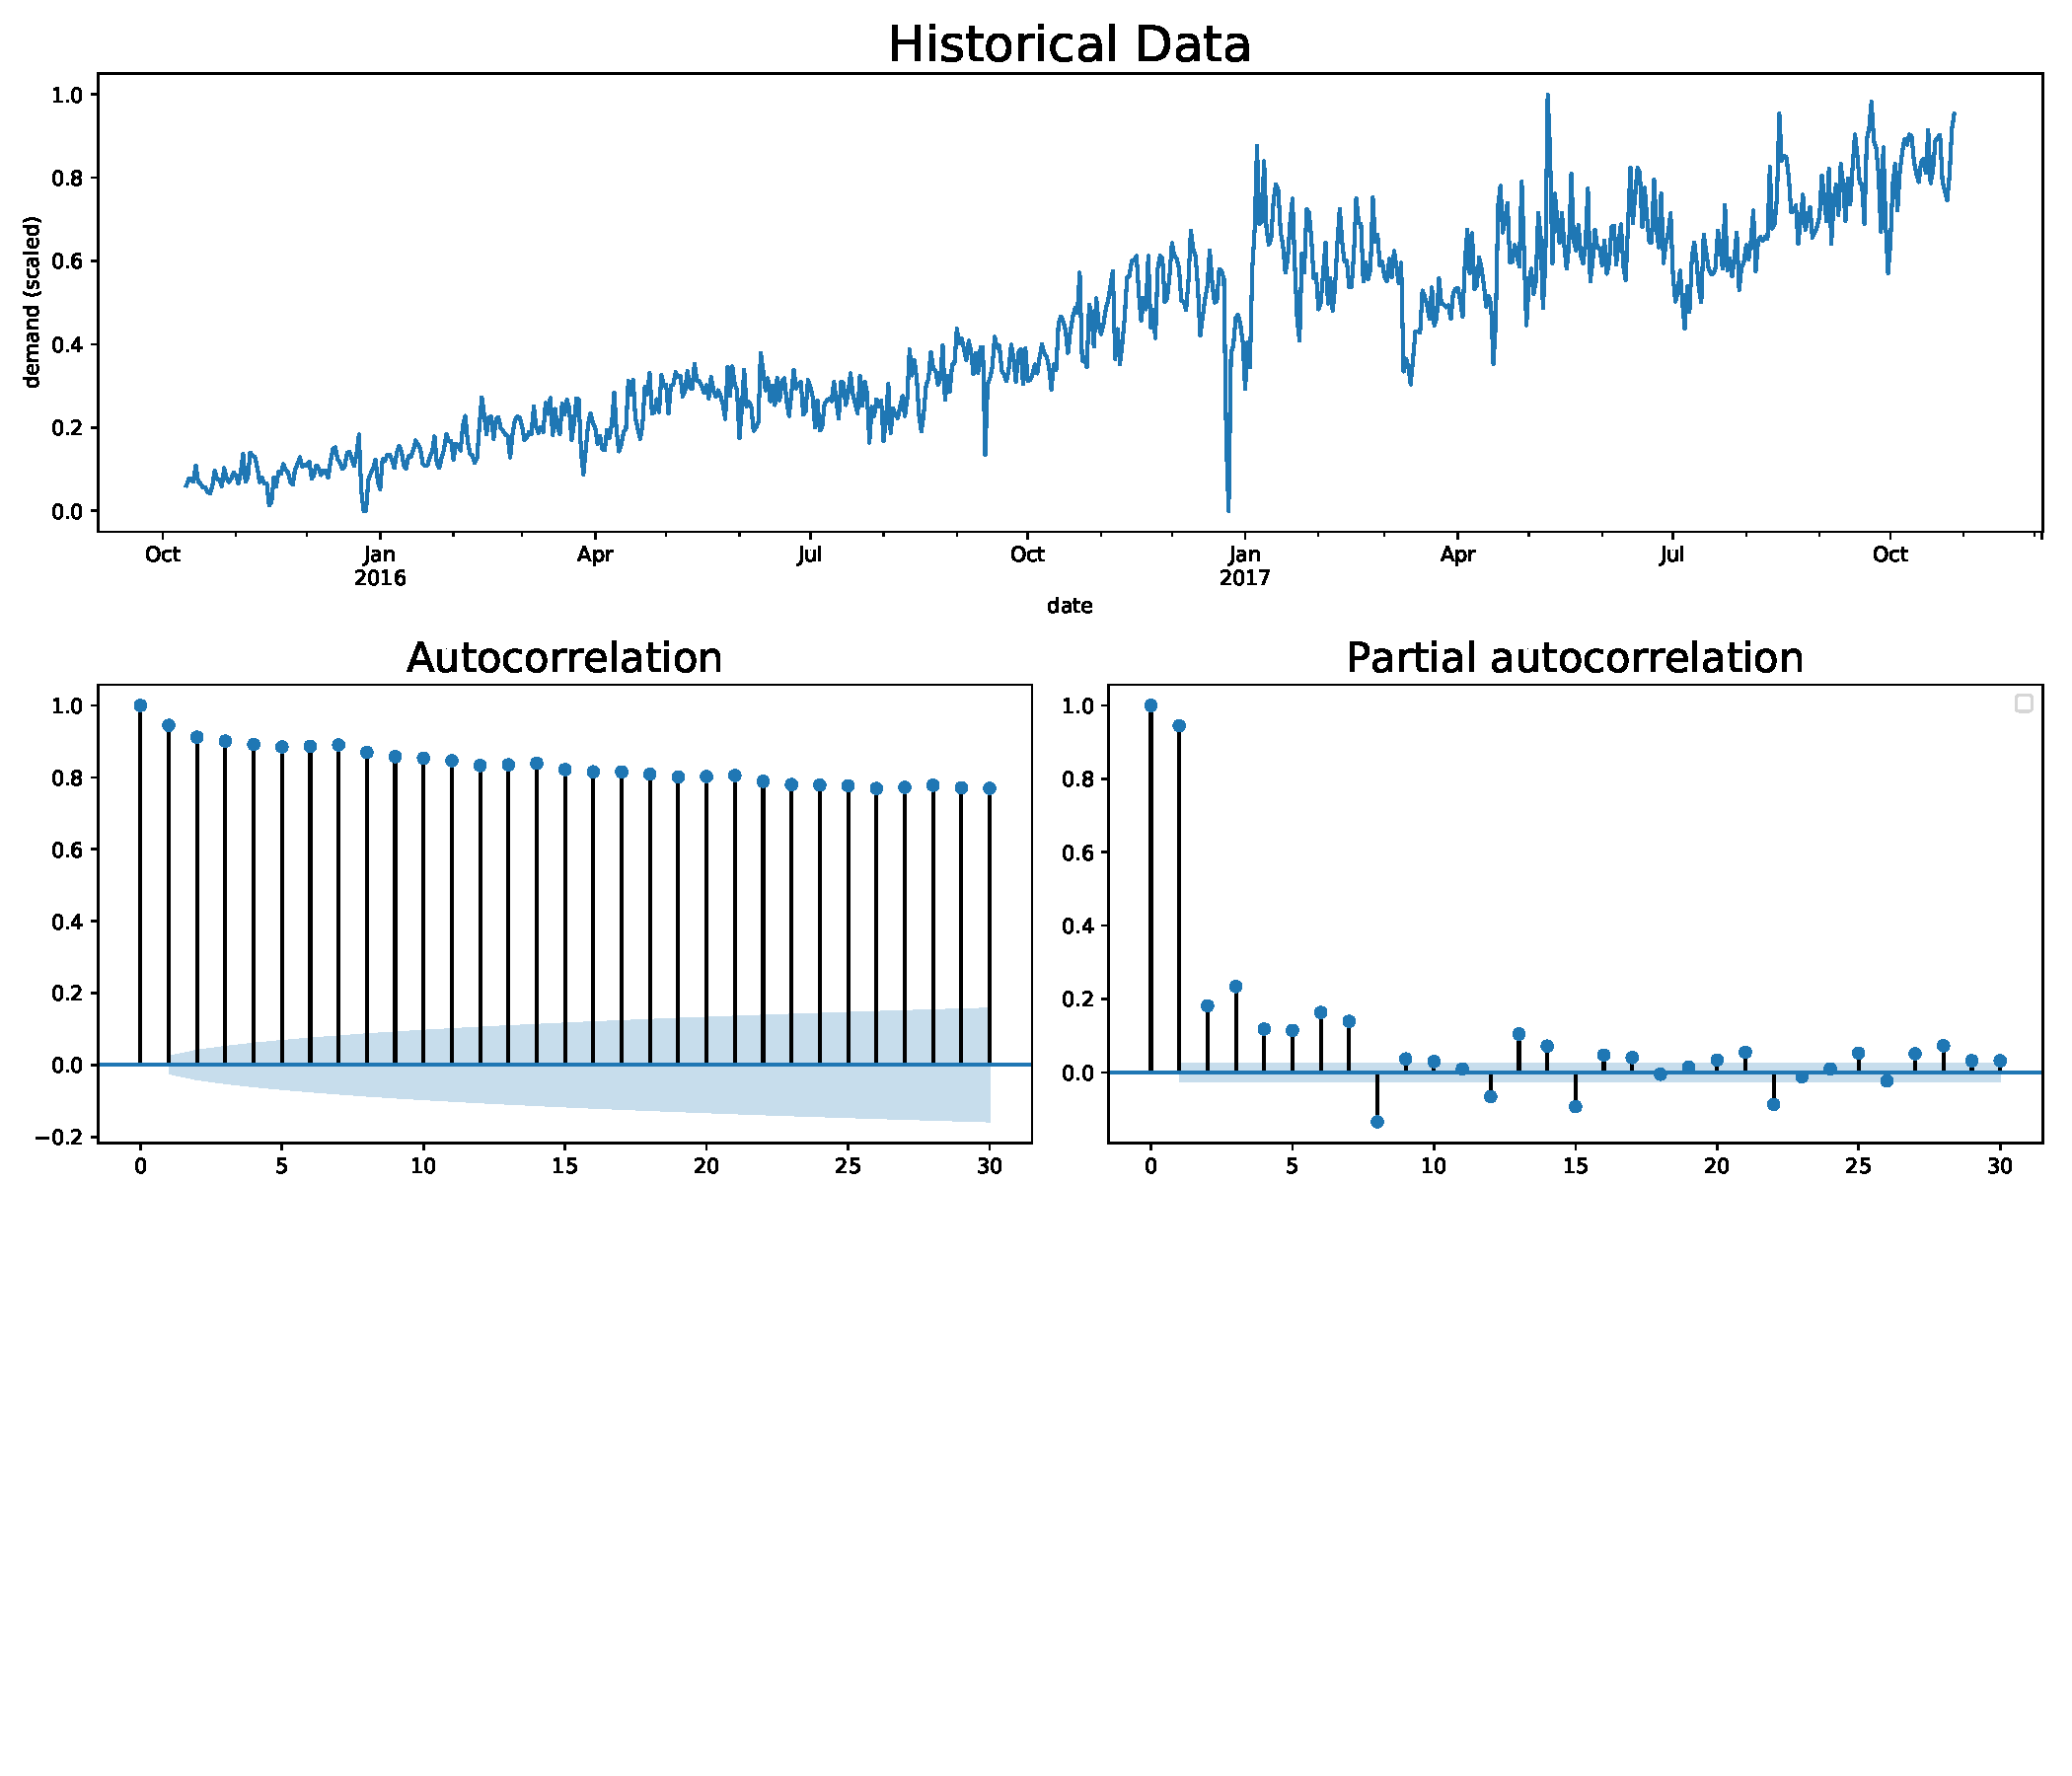
\includegraphics[width=\linewidth]{figures/series_ex.pdf}
  \caption[An example of the provided time-series data]{An example of the provided time-series data, together with correlation plots}
  \label{fig:exploratory}
\end{figure}


\subsubsection{Exponential smoothing model}
The second model we decided to include in our prediction module is the exponential smoothing model, as it is easily interpretable and the parameter selection is straightforward and fast. In the exploratory analysis section, we have shown that the provided data contain signs of weekly seasonality and has increasing trend. Therefore it might seem that the Holt-Winters method as introduced in section \ref{intro_exp} might be suitable. However, instead of using the regular Holt-Winters method, we initially decided to use multiple seasonality extension of the method similar to the one used in \cite{shahin2017using} so that the model could account for weekly, monthly and yearly seasonalities. After we have performed some preliminary benchmarks, we found out that the monthly seasonality component did not improve the results, so the final model is based on ``double seasonal additive exponential smoothing method", and is formulated as follows:

\begin{equation}
\begin{gathered}
\begin{aligned}
\hat{y}_{t+h|t} &= l_t + h b_t^{(h\phi)} + w_{t-m_1 + h} + r_{t-m_2 +h} \\
l_t &= \alpha (y_t - w_{t-m_1} - r_{t-m_2}) + (1-\alpha)(l_{t-1} + b_{t-1}) \\
b_t &= \beta(l_t - l_{t-1}) + (1-\beta) b_{t-1} \\
w_t &= \gamma_{w}(y_t - l_{t-1} - r_{t-m_2}) + (1-\gamma_{w}) w_{t-m_1} \\
r_t &= \gamma{r}(y_t - l_{t-1} - w_{t-m_1}) + (1-\gamma_{r}) r_{t-m_2}
\end{aligned}
\end{gathered}
\end{equation}
Where $\hat{y}_{t+h|t}$ is the h steps ahead forecast from time step t,
$l_t$ denotes the level component at time step t, $b_t$ is the trend estimate at time step t, $w_t$ is the weekly seasonality component at time step t, $r$ the yearly seasonal component, $\alpha$ is the level smoothing coefficient, $\beta$ is a trend smoothing coefficient, $\gamma_w$, $\gamma_r$ are smoothing parameter of the weekly and seasonality components. The parameters $m_1$, $m_2$ denote the periodicity of the seasonal components, so $m_1$ = 7 is the periodicity of the weekly component, $m_2$ = 365 of the yearly component. Another parameter is $\phi$, which is a trend damping parameter. We decided to include it, so that it prevents longer term forecast to be strongly affected by the last trend estimate, which often happened in the preliminary phase of research. 

The initial values of $l_0$ is selected as the first value in the time-series training data, $b_0$ is selected as the difference between the first two values in the series, $w_0$  $r_0$ are set to the mean difference between the first value and the values in the first period of the seasonality component.

For the coefficient selection, we use L-BFGS \cite{bfgs} method, which is a optimization algorithm for parameter selection. During the training, for every parameter set, the SSE error is computed for forecasting in last three periods from the end of the training series, each period has the same length as the future forecasting period, each time all data before the period is used to tune the model components.


\subsection{Scenario generation}
\label{sec:approach_scenario}
So far, we have described the used demand forecasting algorithms. In this section we describe our scenario generation procedure for our stochastic inventory models.

Once we have fitted any model described in section \ref{sec:approach_prediction}, we obtain the following:

\begin{itemize}
\item The forecasts $x_1,\dots,x_T$ where $x_i$ is a forecast for future timestep i and T is the forecasting horizon
\item The model residuals $\{e_{1},\dots,e_{L}\}$. Where each residual value is obtained from the difference $e_{j} =
y_{j}-\hat{y}_{j}$, which is the difference between the actual values at time step j denoted $y_{j}$ and the fitted values $\hat{y}_{j}$, and L is the number of time steps in training data.
\end{itemize}

From the residuals, we compute their standard deviation estimate $\sigma$, and we sample ``errors'' from $\mathcal{N}(0, \sigma^2)$ which are added to the forecasts.


\subsection{Inventory control}
\label{sec:sol_inopt}
In previous sections, we have shown the proposed demand predictors and instructions on how to generate set of demand scenarios from these predictions. In this section we describe our inventory model, whose input is the set of scenarios and the output is the ordering policy for next periods.


We will formulate our solution using stochastic programming as we expect our models to account for demand uncertainty. More specifically, the solution will be based on the Multi period Newsvendor model, as the formulation is very flexible and allows us to further extend it to create more precise model for purposes of our task.

In section \ref{sec:inopt_theory} we have provided an introduction to multi stage stochastic models, which are built on the assumption that we can make the decision for each time stage right before the time stage. However, our solution is based on \textbf{multi period} modeling approach, which differs from multi stage models by its assumption that all decisions are made already before the first stage. 

\subsubsection{Base linear program}
As we have already stated, our solution is based on the stochastic Newsvendor model. The uncertainty of the solution is represented by a set scenarios and their respective probabilities and the set of decisions is obtained by solving a linear program. In section \ref{sec:inopt_theory} we have shown the linear program for the base multi stage Newsvendor model. Considering the differences between the assumptions of the multi stage and multi period models, we can state the linear program for the multi-period Newsvendor as follows: 

\begin{equation}
\label{eq:period_nw}
\begin{gathered}
\min_{x_{t}} \quad 
\sum\limits_{k=1}^{K}{ p_k \sum\limits_{t=1}^{T}{ z_{k,t} }} \\
\begin{aligned}
\textup{s.t.}\quad  & z_{k,t}  \geq (c_t-b_t)x_{t} + b_t d_{t} - b y_{k,t} ,\ k = 1,\dots,K,\  t = 1,\dots,T\\
                  & z_{k,t}  \geq (c_t+h_t)x_{t} - h_t d_{t} + h y_{k,t} ,\ k = 1,\dots,K,\  t = 1,\dots,T  \\
        & x_{t} \geq 0,\  t = 1,\dots,T\\ 
        &  y_{k,t+1} = x_{t} + y_{k,t} - d_{k,t},\  t = 1,\dots,T\\
\end{aligned}
\end{gathered}
\end{equation}
Where $c_t$, $h_t$, $b_t$ are the per unit ordering, holding and shortage costs at time stage t, $d_{k,t}$ is the demand at time stage t under scenario k, $p_k$ is probability of scenario k, $x_{t}$ is ordered amount for time stage t, $y_{k,t}$ is expected leftover inventory from stage t-1 under scenario k, $z_{k,t}$ is expected cost at time stage t under scenario k.

We will use this mixed integer linear program as a base for our final solution.

\subsubsection{Linear program extensions}
Even though the proposed linear program \ref{eq:period_nw} allows us to obtain the ordering amounts by optimizing some sort of expected cost, it does not fully capture the real world retailer's case, as it, for instance, does not account for goods deterioration. For this reason, we have to add the following necessary extensions to the base linear program:

\begin{itemize}
\item \textbf{Disallow back orders:} Because we are modeling am online grocery store, we have to remove the possibility of back orders (back order is a case of unsatisfied demand at some period satisfied in later period) in from the model, as back orders are not supported by the shop. Therefore, we have to update the constraint $y_{k,t+1}\ =\ x_t - d_{k,t}$ and replace it with $y_{k,t+1}\ =\ max(0, x_t - d_{k,t})$. Such constraints are commonly added to linear programs using the \textit{big M method}, which is also recommended by the solver used by this study, Gurobi 8.0.0 \cite{gurobi}, if the M constant is as small as possible. Therefore, we will replace the original constraint with the following:

\begin{equation}
\begin{gathered}
\begin{aligned}
 y_{k,t+1}\ &\geq x_t + y_{k,t} - d_{k,t},\  t = 1,\dots,T\\ 
  y_{k,t+1}\ &\geq 0,\  t = 1,\dots,T\\ 
   y_{k,t+1}\ &\leq x_t + y_{k,t} - d_{k,t} + M(1-b),\  t = 1,\dots,T\\  
   y_{k,t+1}\ &\leq Mb,\  t = 1,\dots,T\\ 
 \end{aligned}
\end{gathered}
\end{equation}
Where b is an additional binary variable and M is constant, either equal to maximum inventory level (if available),
or to multiple to daily maximum demand in all scenarios.

\item \textbf{Per order fixed costs:}
The base linear program only includes per unit ordering costs, although it is quite common that suppliers charge per order costs as well. Therefore, we add the following constraint:

\begin{equation}
\begin{gathered}
\begin{aligned}
 x_{t}\ &\leq w_{t}M,\  t = 1,\dots,T \\
 \end{aligned}
\end{gathered}
\end{equation}
Where $w_{t}$ is binary variable indicating that order will be placed at time stage t. We also have to update the objective to include the per order costs:
\begin{equation}
\min_{x_{t}} \quad 
\sum\limits_{k=1}^{K}{ p_k \sum\limits_{t=1}^{T}{ z_{k,t} }} + \sum\limits_{t=1}^{T}{f_{t} w_{t} }
\end{equation}
Where $f_{t}$ is the per order cost at time stage t.

\item \textbf{SKU expiration date:}
Because our target is to generate ordering policies of a grocery online store for multiple weeks ahead, our model is also expected to include item expiration. For simplicity, we assume that the store sells goods in the order they were received, the expired goods are removed from inventory right after expiration, and the expiration date always occurs after fixed interval of \textbf{u} time stages after they are received in stock.
We introduce another set of variables $l_{k, \tau, t}$, which denotes the left over inventory from time stage $\tau$ at time stage t under scenario k. Finally we update the constraints for $y_{k,t}$ and add constraints for $l_{k, \tau, t}$:
\begin{equation}
\begin{gathered}
\begin{aligned}
 y_{k,t+1}\ &\geq x_t + y_{k,t} - d_{k,t} -l_{k, t-u, t},\  t = 1,\dots,T-1\\ 
  y_{k,t+1}\ &\geq 0,\  t = 1,\dots,T-1\\ 
   y_{k,t+1}\ &\leq x_t + y_{k,t} - d_{k,t} -l_{k, t-u, t} + M(1-b) ,\  t = 1,\dots,T-1\\  
   y_{k,t+1}\ &\leq Mb,\  t = 1,\dots,T-1\\ 
    y_{k,t+1}\ &= \sum\limits_{\tau=t-u}^{t}{ l_{k,\tau,t} },\  t = 1,\dots,T-1 \\
    l_{k,t,t} &\leq x_{k,t},\  t = 1,\dots,T-1 \\
    l_{k,\tau,t+1} &\leq l_{k,\tau,t},\  t = 1,\dots,T-1, \ \tau = 1, \dots, T-1 \\
 \end{aligned}
\end{gathered}
\end{equation}


\end{itemize}
\newpage
\subsubsection{Final linear program}
\label{sec:finallp}
After adding all the extensions mentioned above, we obtained this final mixed integer linear program: 

\begin{equation}
\label{eq:final_nw}
\begin{gathered}
\min_{x_{t}} \quad 
\sum\limits_{k=1}^{K}{ p_k \sum\limits_{t=1}^{T}{ z_{k,t} }} + \sum\limits_{t=1}^{T}{f_{t} w_{t} } \\
\begin{aligned}
\textup{s.t.}\quad   z_{k,t}  &\geq (c_t-b_t)x_{t} + b_t d_{t} - b y_{k,t} ,\ k = 1,\dots,K,\  t = 1,\dots,T\\
                   z_{k,t}  &\geq (c_t+h_t)x_{t} - h_t d_{t} + h y_{k,t} ,\ k = 1,\dots,K,\  t = 1,\dots,T  \\
         x_{t} &\geq 0,\  t = 1,\dots,T\\ 
         x_{t}\ &\leq w_{t}M,\  t = 1,\dots,T \\
  y_{k,t+1}\ &\geq x_t + y_{k,t} - d_{k,t} -l_{k, t-u, t},\  t = 1,\dots,T-1\\ 
  y_{k,t+1}\ &\geq 0,\  t = 1,\dots,T-1\\ 
   y_{k,t+1}\ &\leq x_t + y_{k,t} - d_{k,t} -l_{k, t-u, t} + M(1-b) ,\  t = 1,\dots,T-1\\  
   y_{k,t+1}\ &\leq Mb,\  t = 1,\dots,T-1\\ 
    y_{k,t+1}\ &= \sum\limits_{\tau=t-u}^{t}{ l_{k,\tau,t} },\  t = 1,\dots,T-1 \\
    l_{k,t,t} &\leq x_{k,t},\  t = 1,\dots,T-1 \\
    l_{k,\tau,t+1} &\leq l_{k,\tau,t},\  t = 1,\dots,T-1, \ \tau = 1, \dots, T-1 \\
 \end{aligned}
\end{gathered}
\end{equation}


\subsubsection{Decomposition}
It can be easily seen that our final final mixed integer linear program is quite complex. For illustration, a testing problem with three week planning horizon (21 time stages) and 100 scenarios has over 15000 variables. On the testing machine with Intel Core i7 7700HQ and 24 Gigabytes of RAM, the Gurobi optimizer found the optimal solution after more than 15 minutes, you can see results of an experiment with the running time rate of growth in figure \ref{fig:ext_runtime}. The task of the model in the experiment was to iteratively create inventory policy, while considering 5,10,20,40,60 and finally 80 scenarios. The running time for 80 scenarios that can be seen in the graph is not the actual running time. As the inventory policy generation took more than the 2 hour time limit, it was stopped before generating an optimal solution. The experiment therefore did not reject our hypothesis that the order of growth is exponential in number of scenarios. Considering that companies would likely need to create ordering policies for thousands of products, we decided to implement one of decomposition approaches introduced in section \ref{sec:nwi}, the Progressive Hedging Algorithm. This decomposition methods improves the running time of the model, and allows us to use the model with more demand scenarios, which can further improve its performance, as can be seen in section \ref{sec:eval}.

\begin{figure}
  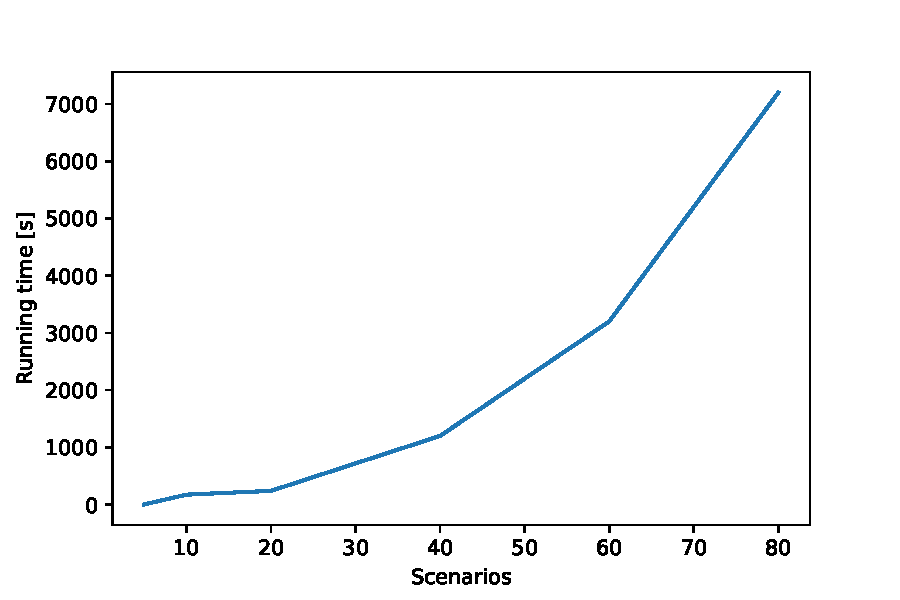
\includegraphics[width=\linewidth]{figures/running_time.pdf}
  \caption[Experiment with extensive form running time]{Experiment with extensive form running time.}
  \label{fig:ext_runtime}
\end{figure}

Progressive hedging algorithm's idea is straightforward, it decomposes the extensive form of a multi stage problem by scenarios in a set of smaller problems. The scenario subproblems are modified with a penalization term, which measures the deviation of the scenario solution from the scenario invariant solution.
Even though convergence to globally optimal solution in the mixed integer programming case is not guaranteed, researchers have shown that the algorithm can find high quality solutions \cite{gade2016obtaining}. Another difficulty arises with selection of penalty parameters and converge acceleration techniques, however researchers such as. Watson et al. \cite{watson2008progressive} provide ways around these problems.

To clarify, PHA is commonly used only for multi stage problems and the penalization terms are used to force non-anticipativity constraints. Even though our problem is a multi period model and does not contain any non-anticipativity constraints, we will use the penalty terms to enforce that the ordering policies $(x_{k,1},\dots,x_{k,T})$ generated by solving the subproblems converge to the scenario invariant policy $\widehat{x}_{1},\dots,\widehat{x}_{T}$. To include the penalty term, we update the objective function of the subproblem of each scenario \textit{s} to the following:

\begin{equation}
\min_{x_{s,t}} \quad 
\sum\limits_{t=1}^{T}{ z_{t} } + \sum\limits_{t=1}^{T}{f_{t} w_{t} }
+ \sum\limits_{t=1}^{T}{\lambda_{s,t}(x_{s,t} - \widehat{x}_{t})}
+ \frac{1}{2} \sum\limits_{t=1}^{T}{\lambda_{s,t}(x_{s,t} - \widehat{x}_{t})^2}
\\
\end{equation}
Where $\lambda$ is a Lagrange multiplier and $\rho$ is a parameter.

\newpage
The PHA is defined as follows:
\begin{algorithm}
\caption{Progressive Hedging Method for Multi period Newsvendor problem}
\begin{algorithmic}[1]
\State Initialize variables $\rho$, $\gamma$ and $\theta$, set variable k = 0.
 \ForEach{scenario s $\in$ S (set of all scenarios)}
\State solve scenario sub-problem without penalization term
      \EndFor
\State
Set $\widehat{x}_{t}$ = $\sum_{s \in S}{p_s x_{s,t}}, \ t=1,\dots, T$
\State Set $\lambda_{s,t} = \rho_{s}(x_{s, t} - \widehat{x}_{t}),  \ s=1,\dots, |S|, \ t=1,\dots, T$ 
 \ForEach{scenario s $\in$ S }
\State solve scenario sub-problem with penalization term
      \EndFor
\State
Update $\widehat{x}_{t} \gets \sum_{s \in S}{p_s x_s}, \ t=1,\dots, T$
\State Update $\lambda_{s,t} \gets \lambda_{s,t} + \rho_{s}(x_{s, t} - \widehat{x}_{t}),  \ s=1,\dots, |S|, \ t=1,\dots, T$ 
\State Update $\rho \gets \gamma \rho$
\State $\delta_{t} = \frac{ \sqrt[]{\sum_{s \in S}{(x_{s,t} -\widehat{x}_t})} }{ \widehat{x}_t},\ t = 1,\dots, T$
 \For{$t =1,\dots, T$} 
\If {$\delta_{t} \geq \theta$}
return to step 7
\EndIf
\EndFor
\State Terminate.
\end{algorithmic}
\end{algorithm}

The algorithm definition raises a few questions, namely the following: 
\begin{itemize}
\item \textit{The initial value of $\rho$, $\gamma$ and $\theta$:} We have empirically selected the initial value of $\rho = 1$, $\gamma = 1.4$ and $\theta = 0.0001$. The value of $\gamma$ ensures that the value of $\rho$ almost doubles on every second iteration.
\item \textit{Is the termination test on lines 15 - 17 sufficient?} Our simulations have shown that additional tests need to be added. In \cite{watson2008progressive} the authors propose PHA algorithm cycling behavior detection. At each iteration of the algorithm, they save the $x_i$ components of the scenario invariant solution $\widehat{x_1}, \dots, \widehat{x_T}$ using hashing. Once cyclic behavior of any of the decision variables $\widehat{x}_it$ from $\widehat{x_1}, \dots, \widehat{x_T}$ is detected between iterations, its value is fixed to  $max(\widehat{x}_{i,s}), s\in S$.

 We also check the following quantity $\Delta$ at each iteration $k \geq 1$:
\begin{equation}
\Delta = \frac{\sum\limits_{t=1}^{T} \mid \widehat{x}_{k,t} - \widehat{x}_{k-1,t}  \mid }{T}
\end{equation}
Where $\widehat{x}_{k,t}$ denotes the scenario invariant solution at iteration k.
The value of $\Delta$ indicates the mean solution variable change between iterations. If $\Delta \leq \frac{1}{T}$ (means that on average only one variable changed by 1) for 10 consecutive iterations, we terminate the algorithm.

\end{itemize}

\newpage
\section{Evaluation}
\label{sec:eval}
In this section we evaluate both topics of this thesis. For the evaluation purposes, we use the data provided by the supervisor. The evaluation consists of two tasks. First part is dedicated to evaluation of proposed demand forecasting methods, the second contains evaluation of inventory models, primarily with focus on the applicability of an extensive form inventory model and its decomposed form. 

\subsection{General description of our evaluation}
First, we take all the proposed time series prediction models and we benchmark them on 5 selected product classes. Each algorithm has to provide forecasts for 3 periods of length of 28 days. The forecasts are then evaluated using standard accuracy metrics and also visual evaluation is performed. Second, we pick the best performing models, and compare their properties, primarily the residuals.
Afterwards, we pick the model with the best properties, and we use its forecasts and residuals to generate demand scenarios for the inventory models. The inventory models are then benchmarked, every model will generate ordering policies for each of the 3 periods and each product class. Finally, the inventory models are evaluated according to costs associated with their ordering policies.

\subsection{Demand prediction}
\label{sec:dem_eval}
As already mentioned, the evaluation consists of two parts. In this part we evaluate the demand prediction models on a set of 5 product classes (SKU) across 3 consecutive periods of length of 28 days. The periods are the following:
\begin{itemize}
\item From August 1st 2017 to August 28th 2017
\item From September 1st 2017 to August 28th 2017
\item From October 1st 2017 to August 28th 2017
\end{itemize}
Each time a model is tested for given SKU and period, it obtains all historical demand data available before start of the period.

In addition to the models introduced in section \ref{sec:approach_prediction}, we also include the \textit{Prophet}\cite{prophet} model for comparison of accuracies. The Prophet model is a forecasting model developed and used by the company behind the largest social network in the world. The model uses a decomposable time series model of the following form:

\begin{equation}
y_t = g(t) + s(t) + h(t) + \epsilon_t
\end{equation}
Where $y_t$ represents a fitted value at time step t, $g(t)$ is a logistic or linear trend component, $s_t$ is a seasonality component modeled by Fourier series, $h_t$ represents possible effect of holidays and $\epsilon_t$ is is an error term which is assumed to be normally distributed. For finding the model's parameters a L-BFGS \cite{bfgs} algorithm is used.

\subsubsection{Evaluation metrics}
We use mainly two performance measures of forecasting accuracy, root mean squared error and mean absolute percentage error. In general, a forecast error $e$ at is defined as follows:
\begin{equation}
e_i = y_i - \hat{y}_i
\end{equation}
Where $y_i$ is the i-th observation of the time series, and $\hat{y_i}$ is the forecast of the i-th observation.
Root mean squared error (RMSE) is probably the most commonly used scale-dependent measure, it is defined as follows:

\begin{equation}
RMSE = \sqrt[]{\frac{1}{n} \sum\limits_{i=1}^n (e_i)^2 }\end{equation}
The fact that RMSE is scale dependent makes it unsuitable for comparing forecasting performance on different time-series. However, for purposes of anonymization, we actually compute RMSE from scaled values:

\begin{equation}
RMSE = \sqrt[]{\frac{1}{n} \sum\limits_{i=1}^n (\frac{y_i- \hat{y}_i}{m} )^2 }\end{equation}
Where m denotes the maximum observed value in the time-series. This adjustment allows for better comparison across different series. A more common scale-independent forecast error measure is the mean absolute percentage error (MAPE), which describes the error as a percentage value:
\begin{equation}
MAPE = \frac{100}{n} \sum\limits_{i=1}^n \frac{| y_i - \hat{y}_i |}{x_i}
\end{equation}

\subsection{Forecasting evaluation results}
In this part of thesis we discuss the results of evaluation of the proposed forecasting models. Before a general summary, we first discuss the results by each product class in separate subsections.
In each subsection, we provide a summary commentary. In addition to the commentary, each subsection contains a figure showing the product class' demand forecasts, where the forecasts of each model is shown separately, namely the figures \ref{fig:sku1_sep}, \ref{fig:sku2_sep}, \ref{fig:sku3_sep}, \ref{fig:sku4_sep} and \ref{fig:sku5_sep}. In the appendix section \ref{sec:appendix} we also provide figures (\ref{fig:sku1_all}, \ref{fig:sku2_all}, \ref{fig:sku3_all}, \ref{fig:sku4_all} and \ref{fig:sku5_all}) containing the forecasts for each product class, but with the forecasts provided by the models drawn in one plot.
Nonetheless, each of the above mentioned plots also contains part of the time series history preceding the forecasting periods, and the start of each forecasting period is denoted by a dashed line.

We also provide tables with scores of each model in the respective product classes' sections, in addition to these per-product-class results tables, the appendix section \ref{sec:appendix} contains table \ref{tbl:dem_bench}, which contains all scores of all models for every product class.

\newpage
\subsubsection{SKU1 forecasts}
\begin{figure}
\centering
  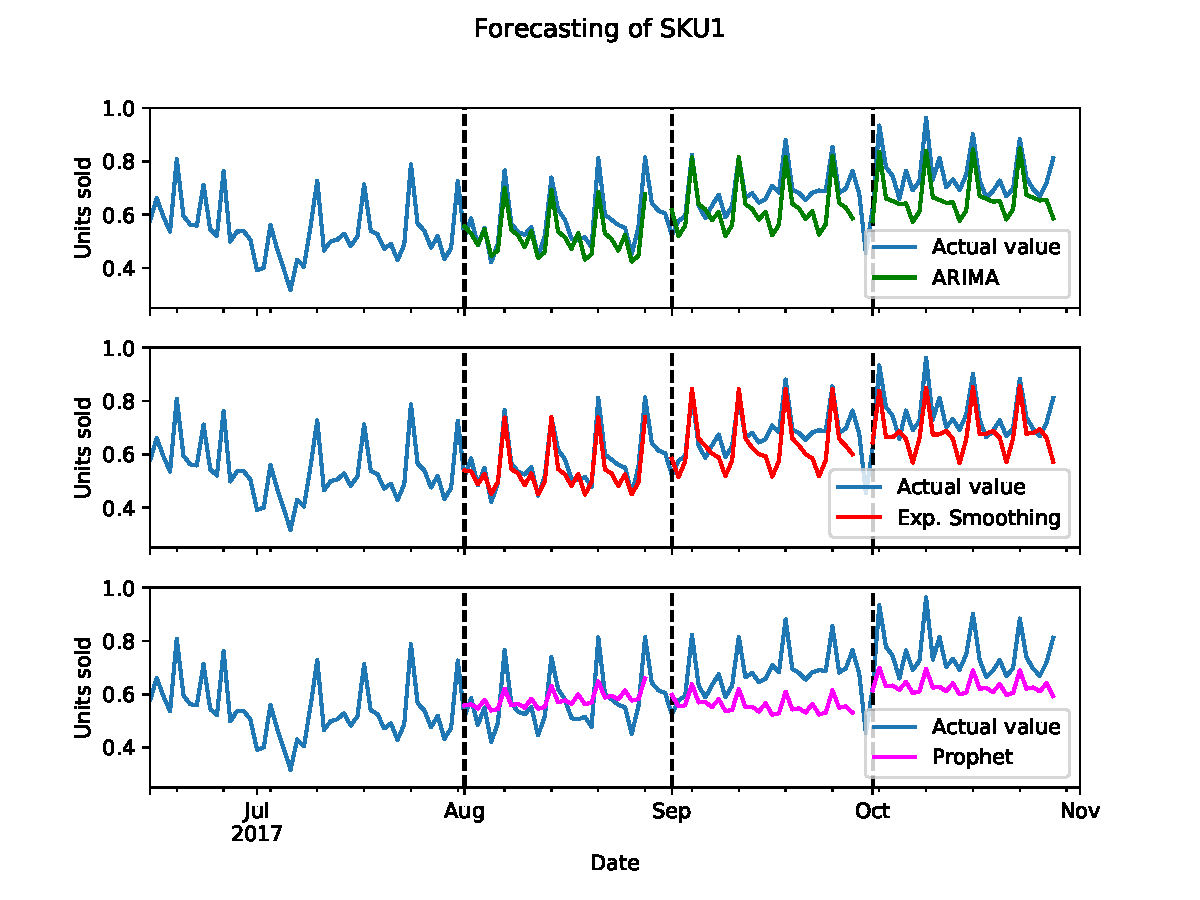
\includegraphics[width=1\linewidth]{figures/SKU1_sep.pdf}
  \caption{Results of first product class - SKU1 forecasting evaluation}
  \label{fig:sku1_sep}
\end{figure}

We first discuss the results of forecasting of the demand of the first product class (SKU1).
The forecasts can be seen in figures \ref{fig:sku1_sep} and \ref{fig:sku1_all} and the RMSE and MAPE scores are in table \ref{tbl:forecast_1}.

\begin{table} \catcode`\-=12
\centering
\begin{tabular}{|l|l|l|l|l|l|l|}
\hline
\multirow{2}{*}{} & \multicolumn{2}{c|}{Exp. Smoothing} & \multicolumn{2}{c|}{ARIMA} & \multicolumn{2}{c|}{Prophet} \\ \cline{2-7} 
                  & MAPE         & RMSE        & MAPE          & RMSE          & MAPE         & RMSE         \\ \hline
Period 1 & \boldmath$5.918$\unboldmath &  \boldmath$0.042$\unboldmath & 8.536 & 0.062 & 10.907 & 0.077   \\ \hline
Period 2 & \boldmath$9.459$\unboldmath &  \boldmath$0.079$\unboldmath & 10.176 & 0.083 & 17.506 & 0.139  \\ \hline
Period 3 & \boldmath$9.327$\unboldmath &  \boldmath$0.087$\unboldmath & 10.917 & 0.095 & 14.426 & 0.129 \\ \hline
\end{tabular}
\caption{Results of SKU1 forecasting}
\label{tbl:forecast_1}
\end{table}

It is clear from both the figure and the table that the best performing models were the ARIMA and exponential smoothing models, which both provide quite similar forecasts, however the smoothing method has slightly better scores. Both models are well adapted for the weekly seasonality in the first period forecast, a little less in the other periods, maybe because they are over-fitted to the seasonality pattern - which has slightly changed in later testing periods. The weekly seasonality adjustment can be seen from the selected order of the (S)ARIMA model - $(0,1,2)x(0,1,1)_7$ in first period and $(1,0,2)x(0,1,1)_7$ in second and third. Also the smoothing model has selected high weekly seasonality smoothing parameter - $\gamma_w$ was higher than 0.4 in all periods. Both models have underestimated the slope of the trend in second and third period, namely the smoothing model in second period, most likely because it selected quite low trend parameter $\beta = 0.06$.
The prophet model's forecasts seem to be adjusted to the seasonality as well, but in somewhat damped way. In the second period, the Prophet model forecasted a decreasing trend, whereas it was actually increasing, which resulted in the worst score.

\newpage
\begin{figure}
  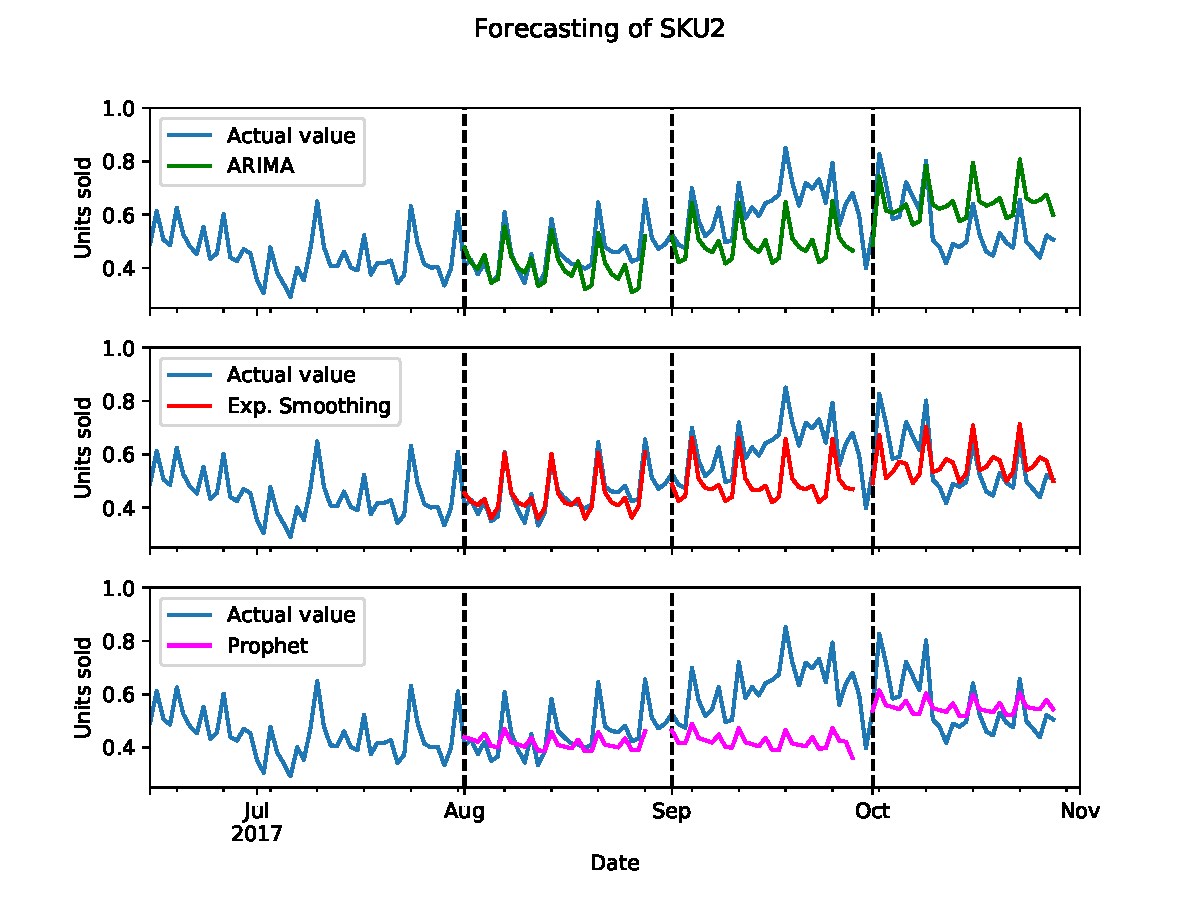
\includegraphics[width=1\linewidth]{figures/SKU2_sep.pdf}
  \caption{Results of second product class - SKU2 forecasting evaluation}
  \label{fig:sku2_sep}
\end{figure}
\subsubsection{SKU2 forecasts}
Product class 2 (SKU2) consists of similar type of products as SKU1, which can be also seen if we compare figures \ref{fig:sku1_sep} and \ref{fig:sku2_sep}. Both the historical data and forecasts show similar patterns. Again, a $(1,0,2)x(0,1,1)_7$ SARIMA model  (this time for each period) was selected. The exponential smoothing method also used similar parameters $\alpha\sim 0.01$,  $\beta\sim 0.9$,  $\phi \sim 0.8$, $\gamma_r \sim 0.04$ and  $\gamma_w \sim 0.4$ to those selected for SKU1. Unfortunately, the models underestimated the trend slope in second period, and the decrease in level in third period as well. This resulted in overall worse scores than the models obtained for forecasting SKU1. 

\begin{table} \catcode`\-=12
\centering
\begin{tabular}{|l|l|l|l|l|l|l|}
\hline
\multirow{2}{*}{} & \multicolumn{2}{c|}{Exp. Smoothing} & \multicolumn{2}{c|}{ARIMA} & \multicolumn{2}{c|}{Prophet} \\ \cline{2-7} 
                  & MAPE         & RMSE        & MAPE          & RMSE          & MAPE         & RMSE         \\ \hline
Period 1 &  \boldmath$6.287$\unboldmath7 &	 \boldmath$0.032$\unboldmath&	10.964&	0.064&	10.455&	0.068	  \\ \hline	
Period 2 &  \boldmath$20.644$\unboldmath &	 \boldmath$0.156$\unboldmath&	20.671&	0.156&	31.996&	0.229  \\ \hline
Period 3 & 14.169 &	0.097&	23.078&	0.130&	 \boldmath$13.094$\unboldmath&	 \boldmath$0.093$\unboldmath	  \\ \hline
\end{tabular}
\caption{Results of SKU2 forecasting}
\label{tbl:forecast_2}
\end{table}




\newpage
\subsubsection{SKU3 forecasts}
Figure \ref{fig:sku3_sep} contains the forecasts for product class 3 (SKU3), which is a class of ham products, the table  \ref{tbl:forecast_3} contains all scores. An ARIMA model of order $(1,1,2)x(1,1,1)_7$ was selected for all periods, which performed well in first and third testing period.
The exponential smoothing method's parameters were selected always a little differently for each period. For first period it was  $\alpha\sim 0.01$,  $\beta\sim 0.95$,  $\phi \sim 0.95$, $\gamma_r \sim 0.04$ and  $\gamma_w \sim 0.34$, for second  $\alpha\sim 0.11$,  $\beta\sim 0.49$, $\phi \sim 0.92$, $\gamma_r \sim 0.04$ and  $\gamma_w \sim 0.42$, and the third  $\alpha\sim 0.17$,  $\beta\sim 0.74$,  $\phi \sim 0.92$, $\gamma_r \sim 0.04$ and  $\gamma_w \sim 0.26$, so the trend and weekly seasonality parameters changed the most, but it always resulted in good scores. On average the Prophet model provided the most accurate forecasts by a slight margin.


\begin{figure}
  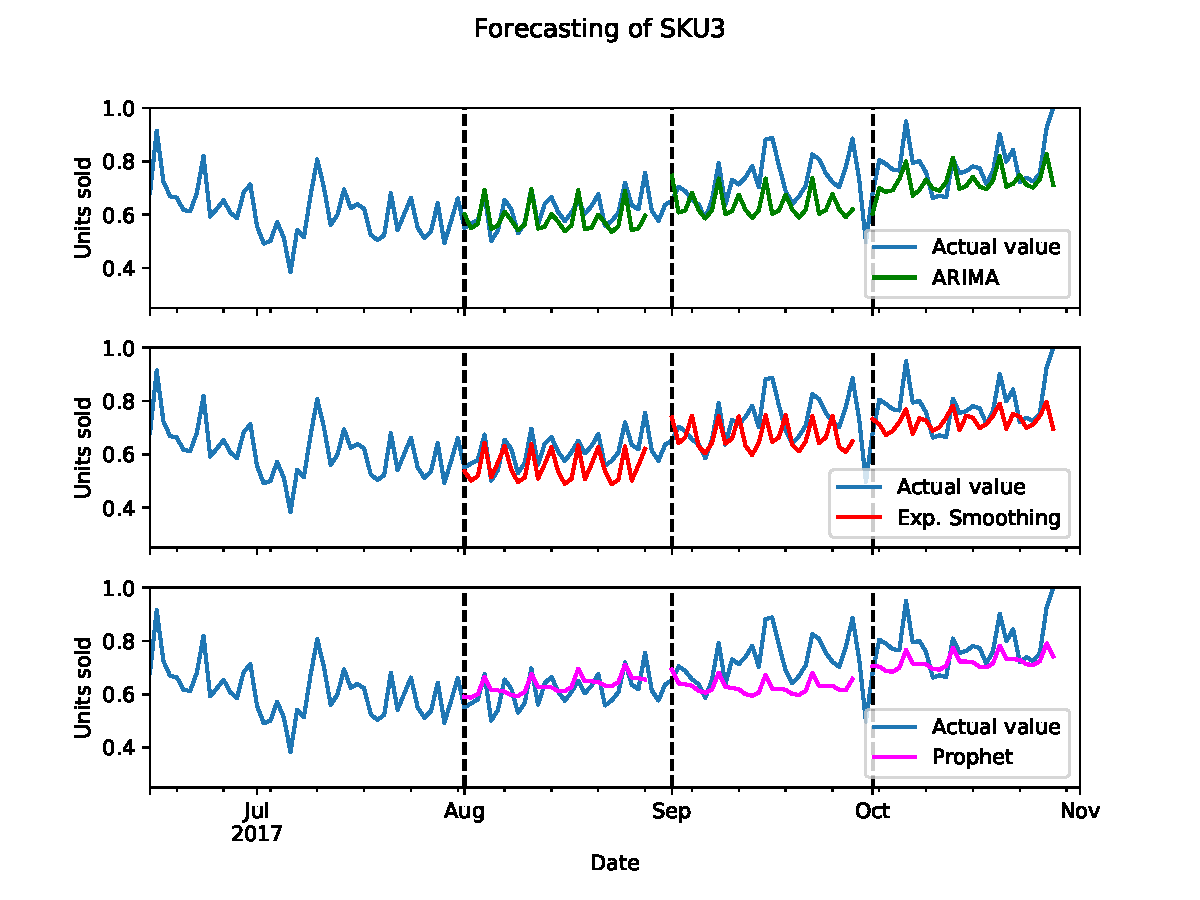
\includegraphics[width=1\linewidth]{figures/SKU3_sep.pdf}
  \caption{Results of third product class - SKU3 forecasting evaluation}
  \label{fig:sku3_sep}
\end{figure}


\begin{table} \catcode`\-=12
\centering
\begin{tabular}{|l|l|l|l|l|l|l|}
\hline
\multirow{2}{*}{} & \multicolumn{2}{c|}{Exp. Smoothing} & \multicolumn{2}{c|}{ARIMA} & \multicolumn{2}{c|}{Prophet} \\ \cline{2-7} 
                  & MAPE         & RMSE        & MAPE          & RMSE          & MAPE         & RMSE         \\ \hline
Period 1 & 10.072 & 0.076 & 7.227 & 0.060 &  \boldmath$6.954$\unboldmath & \boldmath$ 0.052$\unboldmath  \\ \hline
Period 2 &   \boldmath$10.744$\unboldmath &  \boldmath$0.112$\unboldmath & 13.106 & 0.133 & 12.630 & 0.126   \\ \hline
Period 3 & 8.532 & 0.094 & 8.662 & 0.091 &  \boldmath$8.129$\unboldmath &  \boldmath$0.087$\unboldmath  \\ \hline
\end{tabular}
\caption{Results of SKU3 forecasting}
\label{tbl:forecast_3}
\end{table}





\newpage
\begin{figure}
  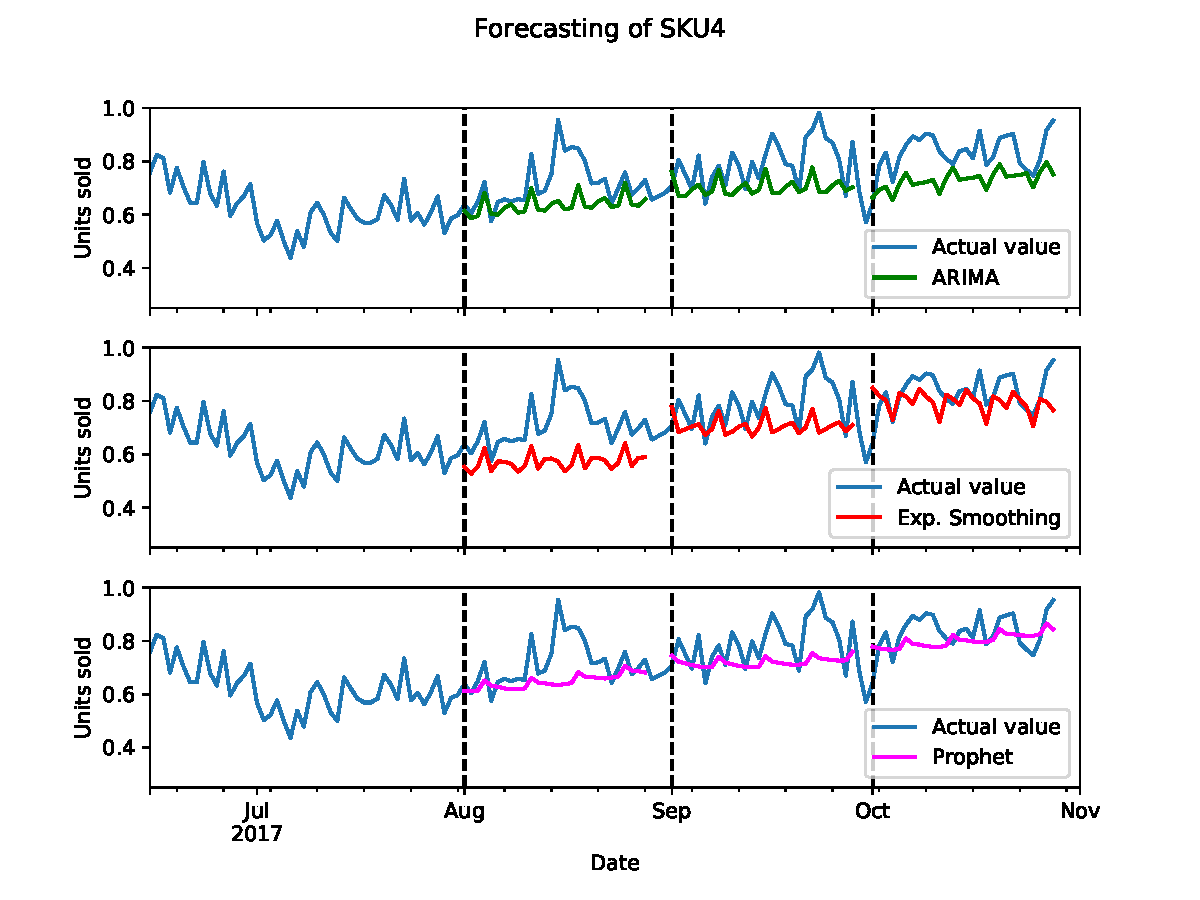
\includegraphics[width=1\linewidth]{figures/SKU4_sep.pdf}
  \caption{Results of fourth product class - SKU4 forecasting evaluation}
  \label{fig:sku4_sep}
\end{figure}

\subsubsection{SKU4 forecasts}
Product class 4 (SKU4) is a class of a hygiene product. From the historical data it seems that the weekly seasonality  pattern is not as significant as in the demand time-series of previous products.
Figure \ref{fig:sku4_sep} contains the plot of forecasts for SKU4  against actual historical data, and the table  \ref{tbl:forecast_4} contains the scores of all models. For SKU4, an ARIMA model of order $(1,0,2)x(0,1,1)_7$ was selected for all periods which seems to follow the slightly increasing trend and the level as well. However the Prophet model's forecasts were more accurate.
The exponential smoothing method provides similar results to both other methods in second and third testing period, but the selected parameters $\alpha\sim 0.01$,  $\beta\sim 0.86$, $\phi\sim 0.8$,   $\gamma_w \sim 0.25$ and  $\gamma_r \sim 0.04$ for first period led to MAPE of almost 20\% .


\begin{table} \catcode`\-=12
\centering
\begin{tabular}{|l|l|l|l|l|l|l|}
\hline
\multirow{2}{*}{} & \multicolumn{2}{c|}{Exp. Smoothing} & \multicolumn{2}{c|}{ARIMA} & \multicolumn{2}{c|}{Prophet} \\ \cline{2-7} 
                  & MAPE         & RMSE        & MAPE          & RMSE          & MAPE          & RMSE         \\ \hline
Period 1  & 19.258 & 0.164 & 10.685 & 0.108 & \boldmath$9.692$\unboldmath & \boldmath$0.106$\unboldmath  \\ \hline
Period 2 & 11.662 & 0.122 & 11.891 & 0.125 & \boldmath$10.561$\unboldmath &\boldmath$ 0.107$\unboldmath \\ \hline
Period 3 & 7.311 & 0.081 & 11.276 & 0.118 & \boldmath$7.139$\unboldmath & \boldmath$0.070$\unboldmath  \\ \hline
\end{tabular}
\caption{Results of SKU4 forecasting}
\label{tbl:forecast_4}
\end{table}



\newpage
\subsubsection{SKU5 forecasts}
We will finish our per-product evaluation with product class 5 (SKU5).
Figure \ref{fig:sku5_sep} contains the plot of forecasts for SKU5  against actual historical data, and the table  \ref{tbl:forecast_5} contains the scores of all models.
 SKU5 is a class consisting of popular drink, which might be the reason why the historical data show a repeating weekly seasonality pattern. In the first testing period, all models seem to fit the seasonality quite well. However in the second testing period the difference between the minima and maxima of the series grew, and there is a slight drop of level at start of September (possibly because the summer holiday ends at that time). None of the models did forecast that. Possibly some product classes would require models adjusted for these ``holiday'' effects.
 For SKU5, an ARIMA models of orders $(1,1,2)x(1,1,1)_7$, $(1,1,1)x(1,1,1)_7$, $(1,1,2)x(0,1,1)_7$ were selected for each period respectively. The ARIMA model $(1,1,1)x(1,1,1)_7$ selected for the second period had the highest MAPE of them, maybe it would have been better if the model selection process (BIC criterion) selected same model for all periods. 
The exponential smoothing method provides similar results to both ARIMA in the first two periods. But the $\alpha\sim 0.32$,  $\beta\sim 0.08$, $\phi\sim 0.95$,  $\gamma_w \sim 0.54$ and  $\gamma_r \sim 0.04$ parameters selected for third period resulted in MAPE of 17.7\%. The parameters show signs of over-fitting as the level component is quite high and the trend component is low. Therefore future work might focus on improvement of the ``training" process for both methods. For the holiday effects, a SARIMAX (Seasonal Arima with External Factors \ref{sec:pred_theory}) model with additional ``holiday'' input might provide better results.
Before we finish the commentary, we can state Prophet model achieved very high MAPE scores in every period.

\begin{figure}
  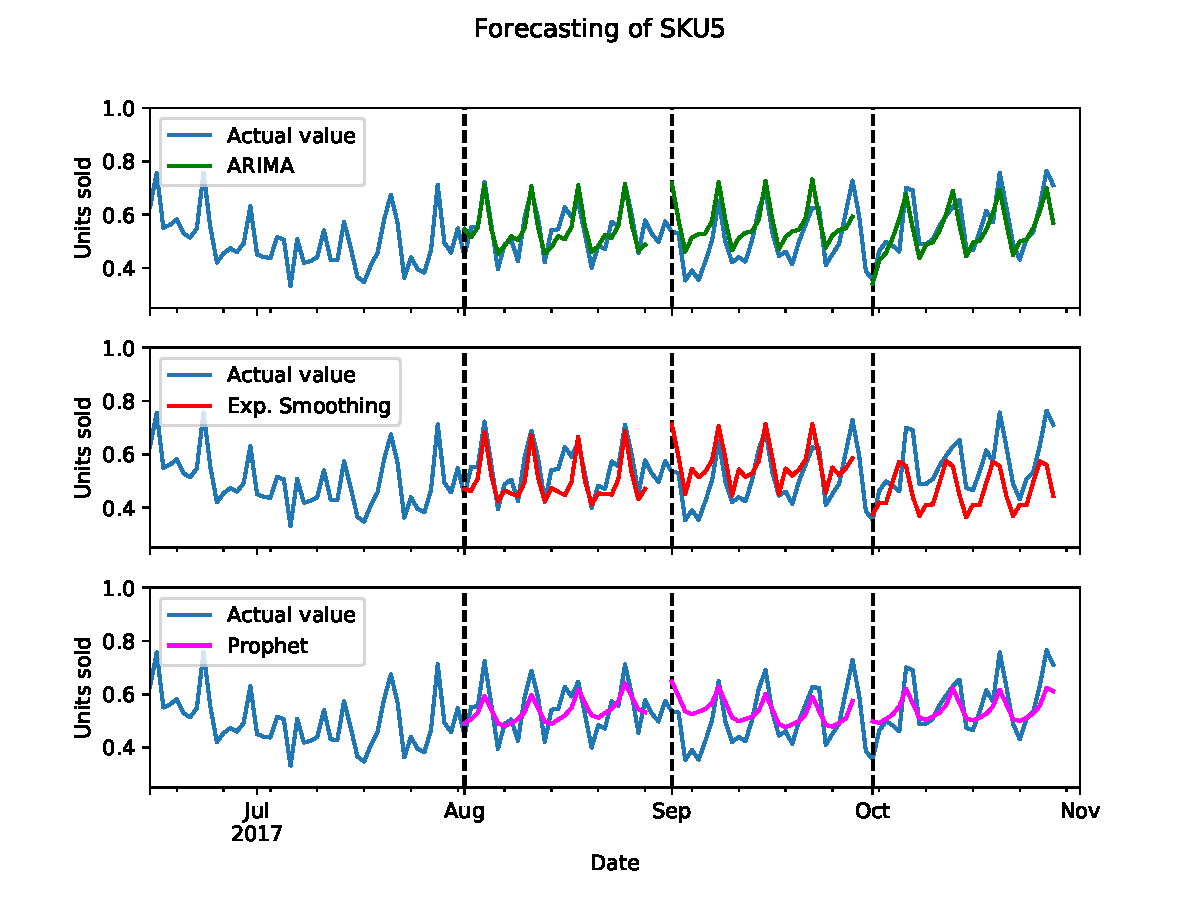
\includegraphics[width=1\linewidth]{figures/SKU5_sep.pdf}
  \caption{Results of fifth product class - SKU5 forecasting evaluation}
  \label{fig:sku5_sep}
\end{figure}


\begin{table} \catcode`\-=12
\centering
\begin{tabular}{|l|l|l|l|l|l|l|}
\hline
\multirow{2}{*}{} & \multicolumn{2}{c|}{Exp. Smoothing} & \multicolumn{2}{c|}{ARIMA} & \multicolumn{2}{c|}{Prophet} \\ \cline{2-7} 
                  & MAPE        & RMSE        & MAPE           & RMSE          & MAPE          & RMSE         \\ \hline
Period 1  &9.438 & 0.067 & \boldmath$7.677$\unboldmath & \boldmath$0.051$\unboldmath & 10.245 & 0.066  \\ \hline
Period 2  & 15.991 & 0.088 & 16.248 & 0.087 & \boldmath$15.372$\unboldmath & \boldmath$0.089$\unboldmath  \\ \hline
 Period 3  & 17.712 & 0.127 & \boldmath$8.320$\unboldmath & \boldmath$0.061$\unboldmath & 9.686 & 0.071  \\ \hline
\end{tabular}
\caption{Results of SKU5 forecasting}
\label{tbl:forecast_5}
\end{table}
\newpage

\subsubsection{Residual analysis}
We will now look at the residuals of the proposed forecasting methods, as we want to generate demand scenarios  for the inventory models using the distribution estimated from the sample mean and sample variance of the residuals. Also the properties of the residuals also provide us with an insight in quality of the model. 
As stated in \cite{hyndman2014forecasting} a well fitted model's residuals have the following properties:

\begin{itemize}
\item The residuals are uncorrelated - if the residuals are correlated, there is some information in the residuals which could be used in the forecasts but were not
\item The residuals have zero mean. If the mean is not zero then then the model is biased (but it can be fixed by shifting the forecasts).
\end{itemize}

For the assessment of possible autocorrelations of the residuals, we can use the autocorrelation plot.  An example of autocorrelation plot can be seen in figure \ref{fig:resid_acf}, which was created from residuals of ARIMA and Exponential smoothing models selected for forecasting the demand in first testing period for SKU1. In the plot we can see that that the residuals of the exponential smoothing model are significantly correlated, whereas the ARIMA model's residuals exhibit almost no correlation.
\begin{figure}
  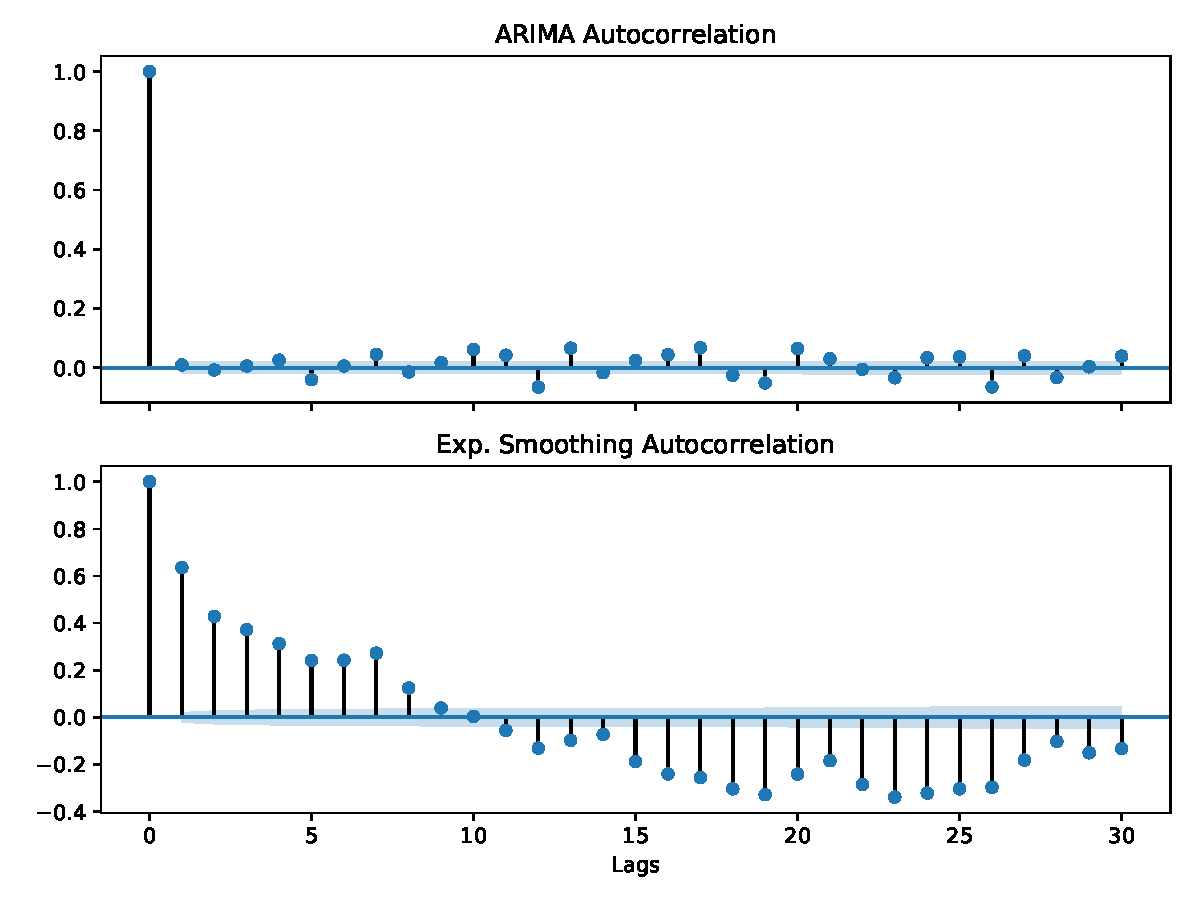
\includegraphics[width=1\linewidth]{figures/autocorrelation.pdf}
  \caption{Autocorrelation plots of residuals of ARIMA and Exponential smoothing models selected for forecasting of SKU1 in first testing period}
  \label{fig:resid_acf}
\end{figure}

Another option of autocorrelation detection is the Ljung-Box test, which may be defined as follows:
\begin{itemize}
\item H0(null hypothesis): The data are independently distributed. 
\item H1(alternative hypothesis): The data are not independently distributed, they exhibit correlation.
\end{itemize}
The test statistic can be computed as follows:
\begin{equation}
Q^* = T(T+2) \sum\limits_{k=1}^h{ (T-k)^{-1} r_k^2}
\end{equation}
Where T is the number of observations, h is the maximum considered lag (\cite{hyndman2014forecasting} suggests $h = 2m$ for seasonal data, where m is the seasonality period), $r_k$ is the autocorrelation at lag k, which is defined as follows:

\begin{equation}
r_k = \frac{\sum\limits_{t=1}^{n-k} (x_t - \overline{x}) (x_{t+k} - \overline{x})}{{\sum\limits_{t=1}^{n}}{ (x_t - \overline{x})^2 }}
\end{equation}
Table \ref{tbl:boxtest} contains the p-values of the Ljung-Box test statistic for first 14 lags computed from residuals of models selected for forecasting of demand in first testing period for all SKUs. According to the table, we can reject the hypothesis that the residuals of the exponential smoothing models are independent. A relatively high p-values of the ARIMA model would suggest that we can't reject the hypothesis that its residuals are independent.
% 10 degress of freedom sig level 5 - chi square 16.8



\begin{table} \catcode`\-=12
\centering
\begin{tabular}{|l|l|l|l|l|l|}
\hline
& SKU1 & SKU2 & SKU3 & SKU4 & SKU5  \\ \hline 
ARIMA & 0.15 & 0.18 & 0.32 & 0.13 & 0.28 \\ \hline
Smoothing & $\sim 0$ & $\sim 0$ &$\sim 0$ & $\sim 0$& $\sim 0$ \\ \hline
\end{tabular}
\caption{Ljung-Box test p-values for lag = 14 of residuals of models used for first period forecasting}
\label{tbl:boxtest}
\end{table}
\newpage

Another important property of the residuals is normality, because our scenario generation approach assumes that the residuals are from normal distribution. For this we will use the Shapiro-Wilk test, which has the null hypothesis that the tested sample comes from normal distribution.
Table \ref{tbl:shapiro_test} contains Shapiro-Wilk test p-values of residuals of models used for first period forecasting. We can see high p-values in the rows of each model, which means the we cannot reject the hypothesis that the residuals are from normal distribution.

\begin{table} \catcode`\-=12
\centering
\begin{tabular}{|l|l|l|l|l|l|}
\hline
& SKU1 & SKU2 & SKU3 & SKU4 & SKU5  \\ \hline 
ARIMA & 0.84 & 0.81 & 0.85 & 0.84 & 0.89 \\ \hline 
Smoothing & 0.90 & 0.87 & 0.91 & 0.85 & 0.94 \\ \hline 

\end{tabular}
\caption{Shapiro-Wilk test p-values of residuals of models used for first period forecasting}
\label{tbl:shapiro_test}
\end{table}
\newpage

\subsubsection{Forecasting evaluation results summary}
We have evaluated the proposed models both visually and using accuracy scores, and we also evaluated the models' residuals using statistical tests. Both our proposed methods performed better than that provided by the Prophet library. The Exponential Smoothing method has the best average accuracy scores, but some of its forecasts had signs of over-fitting. Also the residual auto-correlation evaluation showed the model (or rather the parameter selection) could be further improved. The ARIMA models' average MAPE is slightly higher, but its mean RMSE (computed from scaled series) is exactly same. However, the evaluation has shown that its residuals are likely not correlated and can be from normal distribution. Because of its good ``on average'' performance in all evaluation parts, we have chosen the ARIMA model as the model for generating demand scenarios for the inventory models.

Future research might focus on improving the model selection methods used for selecting the ARIMA models, namely we could theoretically use higher order models. In case of Exponential Smoothing the autocorrelation plots have shown it clearly didn't use some of the information in the historical data.



\subsection{Inventory control}
The next part of our evaluation is dedicated to the inventory control models. In this subsection, we only consider forecasts provided by the best forecasting model according to the evaluation in section \ref{sec:dem_eval} - the ARIMA model, and use it for scenario generation.

During the demand evaluation, the ARIMA model generated forecasts of demand for 5 SKUs across 3 consecutive periods of length of T = 28 days. Each of these forecasts, and the fitted models residuals, are used for demand scenario generation. According to generated scenarios, the models proposed in \ref{eval:models_inv} will output ordering amounts $x_i,\dots, x_T$ for each SKU and each period. The performance of the models is later compared according to costs, which would theoretically be incurred if the inventory policies provided by the models were applied in real world. 

\subsubsection{Models}
\label{eval:models_inv}
In section \ref{sec:sol_inopt} we have designed our extented formulation of the stochastic multi period Newsvendor inventory model. Due to the complexity of its mixed integer linear programming formulation and the computation complexity (especially when used with problem with more stage or scenarios) associated with it, we have suggested that a decomposition approach should be used - the Progressive Hedging Algorithm. Progressive Hedging Algorithm is commonly used for problems that can't be solved in its extensive form in reasonable time, or those that don't fit in RAM. This is not exactly the case of our formulation. As you can see in table \ref{tbl:running_time}, some of the less complex testing problems were solved in a couple of minutes. On the other hand, for some of the problems, the selected Gurobi solver did not provide an optimal solution for the extensive form with only 25 scenarios in under 20 minutes. Considering that an inventory of a store may contain thousands of products, we decided to include the following models in the evaluation, with ``acceptable'' computation time in mind:

\begin{itemize}
\item Extensive form model with 25 scenarios - this model solves the exact formulation problem, but has rather limited amount of information about the possible outcomes of the random demand
\item Progressive hedging model with 250 scenarios - this models solves the decomposed problem, but due to the increased number of scenarios it can hedge against more possible outcomes of the random demand.
\item Base stock model with daily restocking - this model is very simplistic, its only objective is to prevent shortages
\end{itemize}




\subsubsection{Testing parameters}
We will now briefly list the parameters used by the above mentioned models and in the evaluation.

First we can repeat that the planning horizon T of the models is T=28 days. And the goods durability estimates are the following:
\begin{itemize}
\item SKU1 - 4 days as it represents is a fruit product
\item SKU2 - 6 days as it represents a different fruit product
\item SKU3 - 8 days as it represents packaged ham product
\item SKU4 - ``unlimited' durability, as it is a hygiene product which most likely lasts longer than the planning horizon
\item SKU5 - ``unlimited' durability, as it is a packaged drink which most likely lasts longer than the planning horizon

\end{itemize}
Second we list cost types. As we don't know the exact shortage, warehousing and other costs associated with each SKU, we decided to the use the following estimates:

\begin{itemize}
\item Shortage cost - $b_t$: We use a value extracted from the historical data equal to the average daily selling price of the product class
\item Ordering costs (per unit) - $c_t$: we use the values $c_t = 0.65b_t$
\item Fixed ordering costs (per order) - $f_t$: we omitted this cost in evaluation
\item Holding (warehousing) costs (per unit) - $h_t$: we use the values $h_t = \frac{b_t}{50}$
\end{itemize} 
It is clear that the values are very rough estimates and without expert's knowledge our total cost estimates are rather illustrative. 

Now that we have the prices, we can show how we compute the estimated total costs. If we assume that the inventory model required the orders $x_1,\dots,x_T$ and the actual demands were $d_1,\dots,d_T$, then we can calculate the costs as follows:
\begin{itemize}
\item The total shortage cost - $S$: 
\begin{equation}
B = \sum\limits_{i=1}^T b_t max(0, d_i - x_i)
\end{equation}
\item The total ordering cost - $C$: 
\begin{equation}
C = \sum\limits_{i=1}^T c_i x_i 
\end{equation}
\item The total holding cost - $H$: 
\begin{equation}
H = \sum\limits_{i=1}^T h_t max(0, x_i - d_i)
\end{equation}
\item The overall cost V:
\begin{equation}
V = B + C + H
\end{equation}


\end{itemize}

\subsubsection{Total Costs evaluation}
With computation time, the estimated costs is the most important measure when comparing the models mentioned above. The evaluation of the total costs associated withe the orders generated by the models can be seen in table \ref{tbl:costs}, where PHA stands for Progressive Hedging Algorithm, EF for Extensive form. Estimated costs with a star mean that the algorithm did not finish in the time limit of 20 minutes and the result is only the best solution obtained before the limit.

It can be seen that in most cases, both the Newsvendor based models perform better than the simple Base Stock model, sometimes by up to 33\% as in case of testing period 1 for SKU2. This is also reflected in the total sum of costs. PHA model has the lowest sum of estimated costs, EF model is behind by roughly 0.5\%, and the Base Stock model has the largest sum of costs - 12\% higher than PHA.

As the total sum of costs suggest, in most cases the Progressive Hedging model provided the best ordering policy. In only one test case was the EF model's policy better - test period 3 of SKU5. In one test case the Best Stock model had the best result - test case 2 of SKU2, possibly because the forecast had poor accuracy.
From both the total results and the sub-results it seems that the extra information that the PHA model obtained
in the additional scenarios was beneficial enough to outweigh the fact that its just an approximation algorithm of the EF. 

Lets now take a closer look at some of the more interesting test cases.


\begin{table} \catcode`\-=12
\centering
\begin{tabular}{|c|c|c|c|c|c|}
\hline
\multicolumn{3}{|c|}{} &\multicolumn{3}{|c|}{Estimated costs} \\ \hline
\multicolumn{2}{|c|}{}& MAPE &  PHA & EF & Base Stock \\ \hline
\multirow{ 3}{*}{SKU1}& Period 1 & 8.54 & \boldmath $6.6\cdot 10^5 $\unboldmath  & $6.7\cdot 10^5 $ & $7.9\cdot 10^5 $\\  \cline{2-6}
& Period 2 & 10.17 &  \boldmath $7.7\cdot 10^5 $\unboldmath & $7.9\cdot 10^5 $ & $8.6\cdot 10^5 $\\  \cline{2-6}
& Period 3 & 10.91 & \boldmath$8.5\cdot 10^5 $\unboldmath  & $8.7\cdot 10^5 *$ & $9.0\cdot 10^5 $\\ \hline 
\multirow{ 3}{*}{SKU2}& Period 1 & 10.96 & \boldmath$5.7\cdot 10^5 $\unboldmath  & $5.8\cdot 10^5 *$ & $7.3\cdot 10^5 $\\  \cline{2-6}
& Period 2 & 20.67 & $9.2\cdot 10^5 $ & $9.5\cdot 10^5 *$ & \boldmath $8.8\cdot 10^5 $\unboldmath \\  \cline{2-6}
& Period 3 & 23.08 & \boldmath$1.2\cdot 10^6 $\unboldmath  & $1.2\cdot 10^6 *$ & $1.7\cdot 10^6 $\\ \hline 
\multirow{ 3}{*}{SKU3}& Period 1 & 7.23 & \boldmath$1.2\cdot 10^6 $\unboldmath  & $1.2\cdot 10^6 *$ & $1.4\cdot 10^6 $\\  \cline{2-6}
& Period 2 & 13.10 & \boldmath $1.4\cdot 10^6 $\unboldmath  & $1.5\cdot 10^6 *$ & $1.4\cdot 10^6 $\\  \cline{2-6}
& Period 3 & 8.66 & \boldmath $1.5\cdot 10^6 $ \unboldmath & $1.5\cdot 10^6 *$ & $1.6\cdot 10^6 $\\ \hline 
\multirow{ 3}{*}{SKU4}& Period 1 & 10.68 & \boldmath $9.9\cdot 10^5 $\unboldmath  & $9.9\cdot 10^5 $ & $1.0\cdot 10^6 $\\  \cline{2-6}
& Period 2 & 11.89 & \boldmath $1.2\cdot 10^6 $\unboldmath  & $1.2\cdot 10^6 $ & $1.2\cdot 10^6 $\\  \cline{2-6}
& Period 3 & 11.28 & \boldmath $1.4\cdot 10^6 $\unboldmath  & $1.4\cdot 10^6 $ & $1.4\cdot 10^6 $\\ \hline 
\multirow{ 3}{*}{SKU5}& Period 1 & 7.68 & \boldmath $1.7\cdot 10^6 $\unboldmath  & $1.7\cdot 10^6 $ & $2.4\cdot 10^6 $\\  \cline{2-6}
& Period 2 & 16.25 & $1.8\cdot 10^6 $ & \boldmath $1.8\cdot 10^6 $\unboldmath  & $2.4\cdot 10^6 $\\  \cline{2-6}
& Period 3 & 8.32 & \boldmath $1.6\cdot 10^6 $\unboldmath  & $1.7\cdot 10^6 $ & $2.2\cdot 10^6 $\\ \hline 
 \multicolumn{3}{|r|}{Sum }& \boldmath $1.79\cdot 10^7$\unboldmath  & $1.80\cdot 10^7$ & $2.08\cdot 10^7$\\ \hline 
\end{tabular}
\caption{Estimated total costs evaluation}
\label{tbl:costs}
\end{table}

\newpage
We start with test case 2 of SKU1. The policies generated by the PHA model are the best in most cases, however this test case is one of those in which PHA was best by the highest margin. The visualization of the inventory levels can be seen in figure \ref{fig:cost_sku1_p2}.
We can see that at the end of the testing period, the actual demand is slightly higher than the forecasted one, which resulted in multiple periods with shortages of both EF and PHA model. Nonetheless, PHA's policy has significantly less periods with shortages - likely because its solution accounts for more possible demand outcomes. The base stock model has the largest estimated cost due to big amounts of excess inventory.

\begin{figure}
  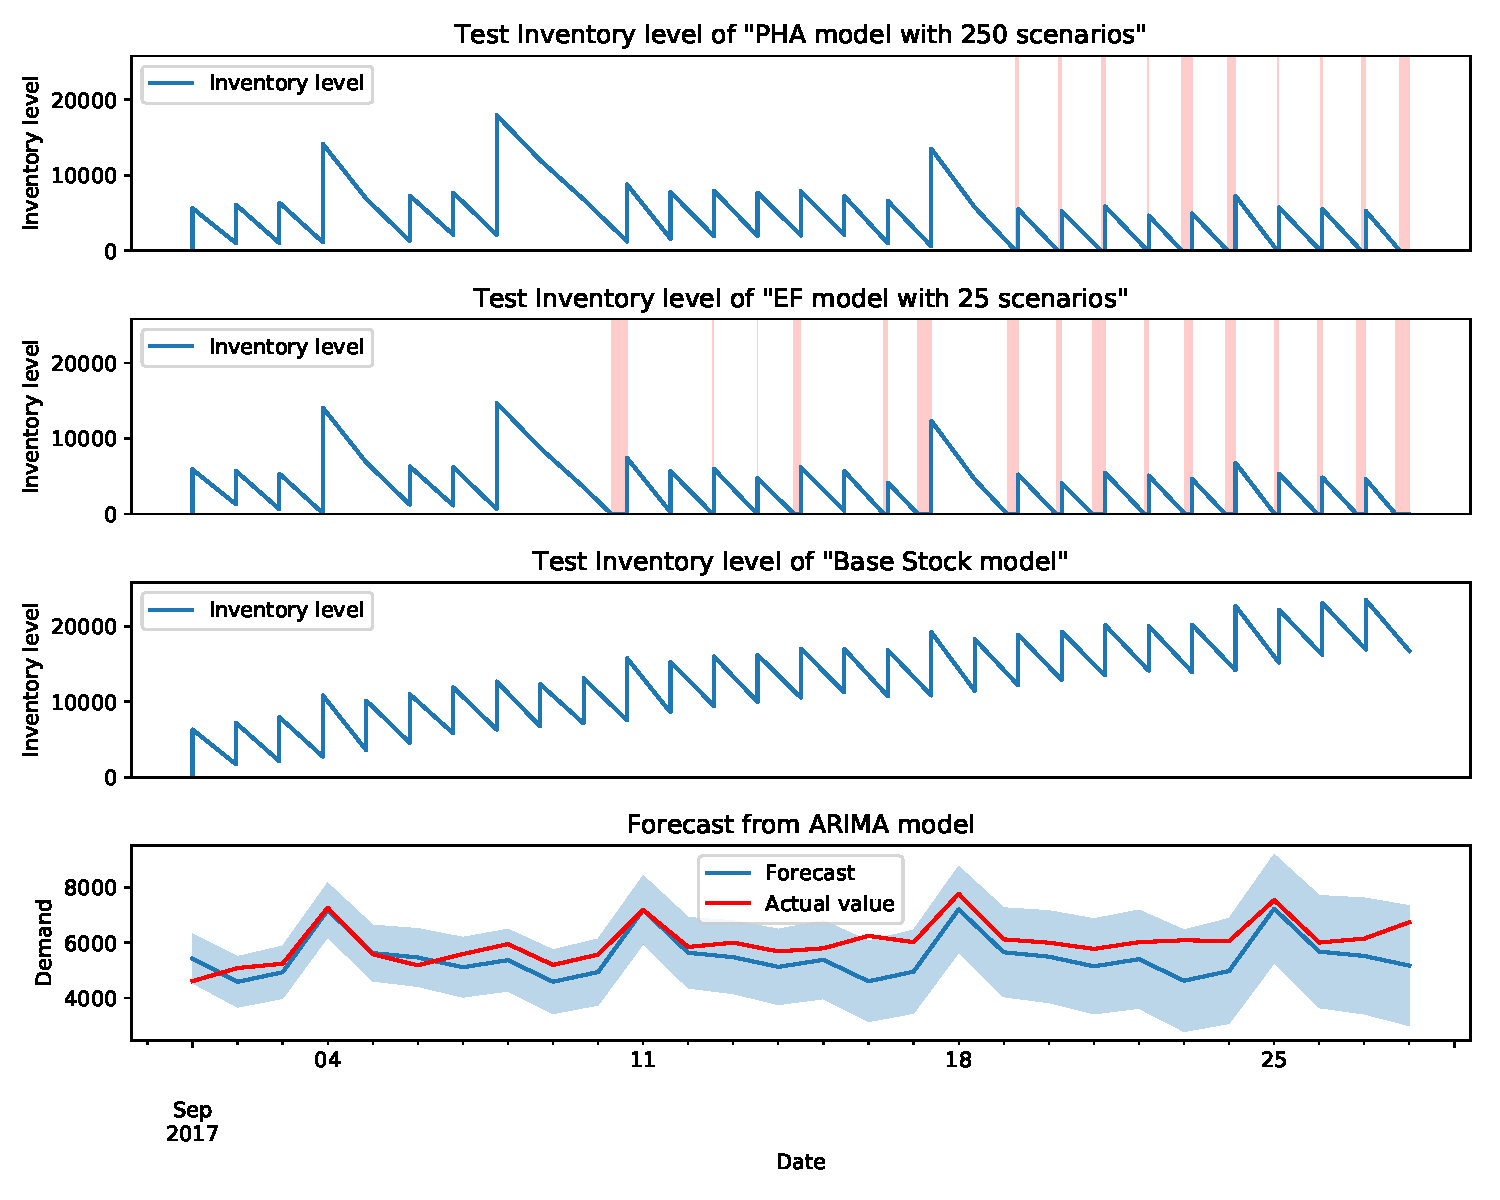
\includegraphics[width=1\linewidth]{figures/cost_sku1_2.pdf}
  \caption[Inventory model simulation visualization for test period 2 of SKU1]{Inventory model simulation visualization for test period 2 of SKU1. The top 3 plots contain inventory level simulations for each model, with periods with shortage highlighted by red rectangles, the bottom plot contains the forecast of ARIMA model with prediction interval in light blue.}
  \label{fig:cost_sku1_p2}
\end{figure}

\newpage


\newpage
%% fixed
We continue with test case 1 for SKU5, as the estimated total cost difference between the Newsvendor based models and the base stock model was highest in this case. PHA model's policy estimated cost was lower by 33\% than that of the base stock model. An inventory simulation of this test case can be seen in figure \ref{fig:cost_sku5_p1}. The large difference between the model's is caused by the accuracy of the forecast (MAPE was 7.7\%). As the base stock model orders the amount equal to the top of the demand prediction interval, it has large amounts of excess inventory in this case. The EF model's policy caused some shortages at the end of the testing period - possibly because the forecasted demand was lower. PHA's policy seems to cover this better, which means it achieved the best result.


\begin{figure}
  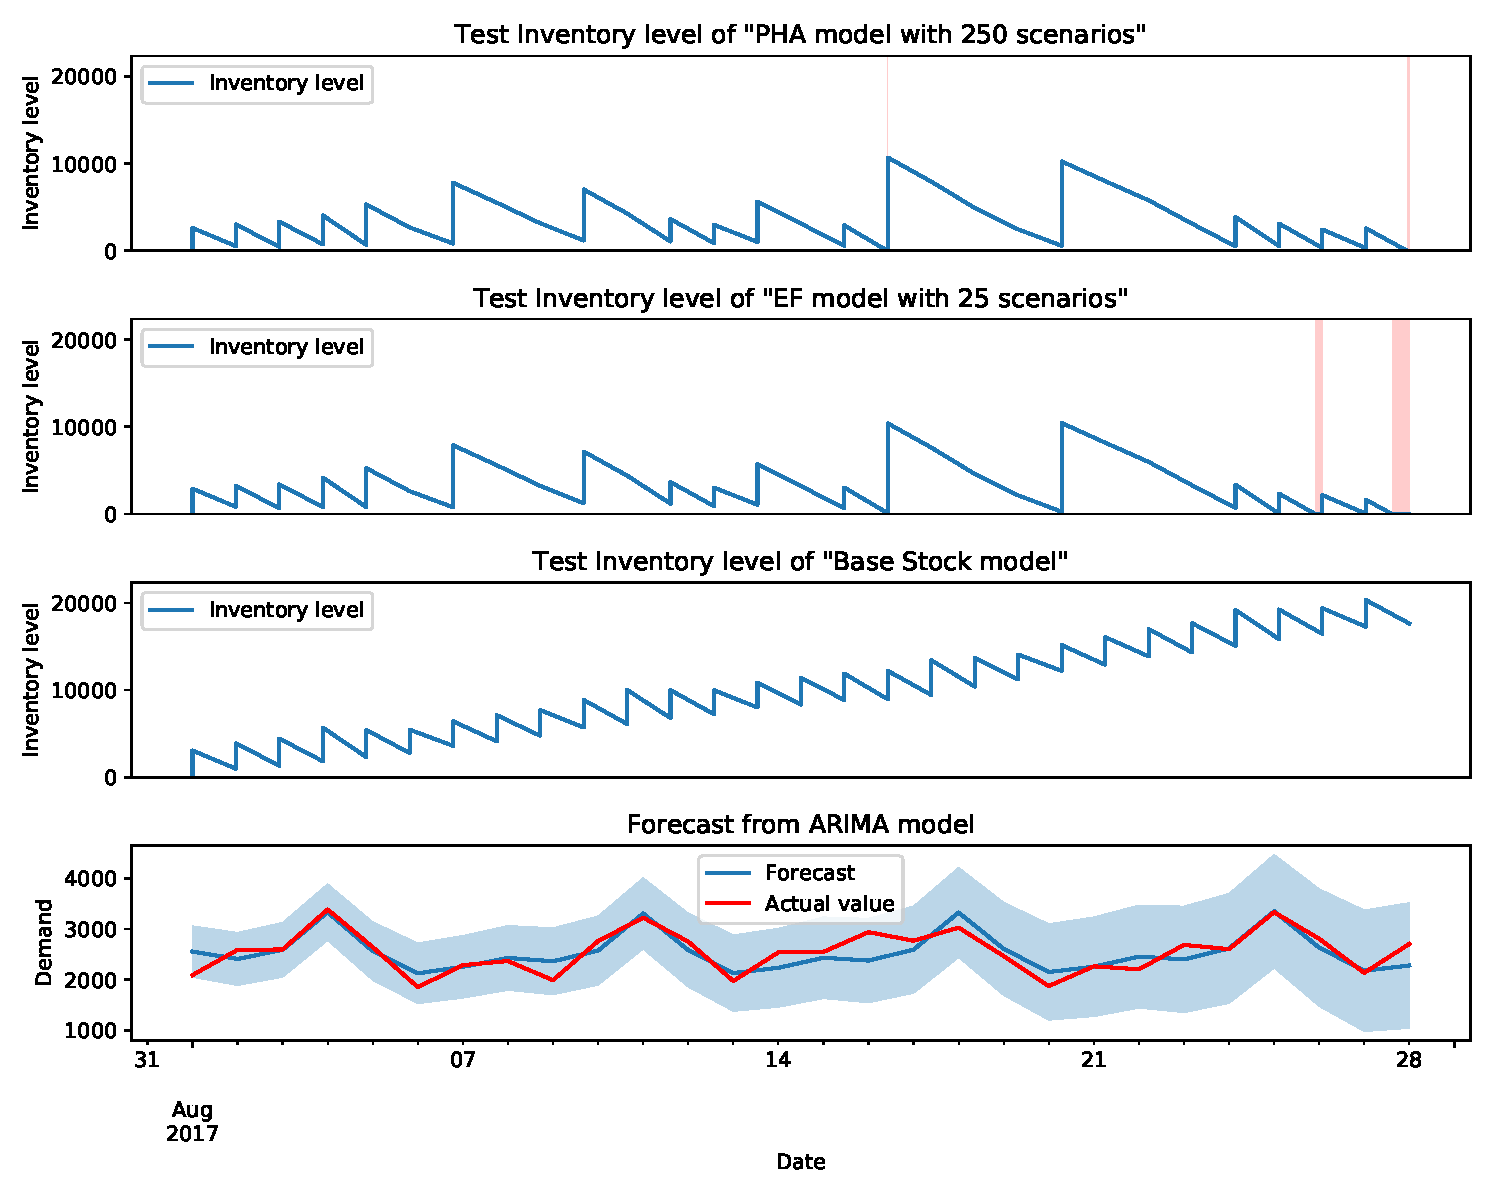
\includegraphics[width=1\linewidth]{figures/cost_sku5_1.pdf}
  \caption[Inventory model simulation visualization for test period 1 of SKU5]{Inventory model simulation visualization for test period 1 of SKU5. The top 3 plots contain inventory level simulations for each model, with periods with shortage highlighted by red rectangles, the bottom plot contains the forecast of ARIMA model with prediction interval in light blue.}
  \label{fig:cost_sku5_p1}
\end{figure}
%% fixed

\newpage


%%%%%% NEW

The next inventory simulation we show in full detail is again for SKU2, this time for test period 2 (figure \ref{fig:cost_sku2_p2}. In this case the base stock model's policy was better than PHA by almost 3\%. For this case, the forecast expected smaller demand (MAPE was almost 21\%). However the top of the prediction interval, which is used as the order amount by the base stock model, aligns with the actual demand quite well for the most part. But during some days in the test period, the demand was so much higher than the expected one that even the base stock model's policy had shortages. Still the shortage costs of base stock model were much lower than that of other models. 

The PHA's more scenarios and its ability to finish processing in the 20 minute time limit (the EF model did not finish in the time limit), have probably helped it to achieve significantly better result than EF, but its estimated costs were still significantly higher then those of base stock model.

\begin{figure}
  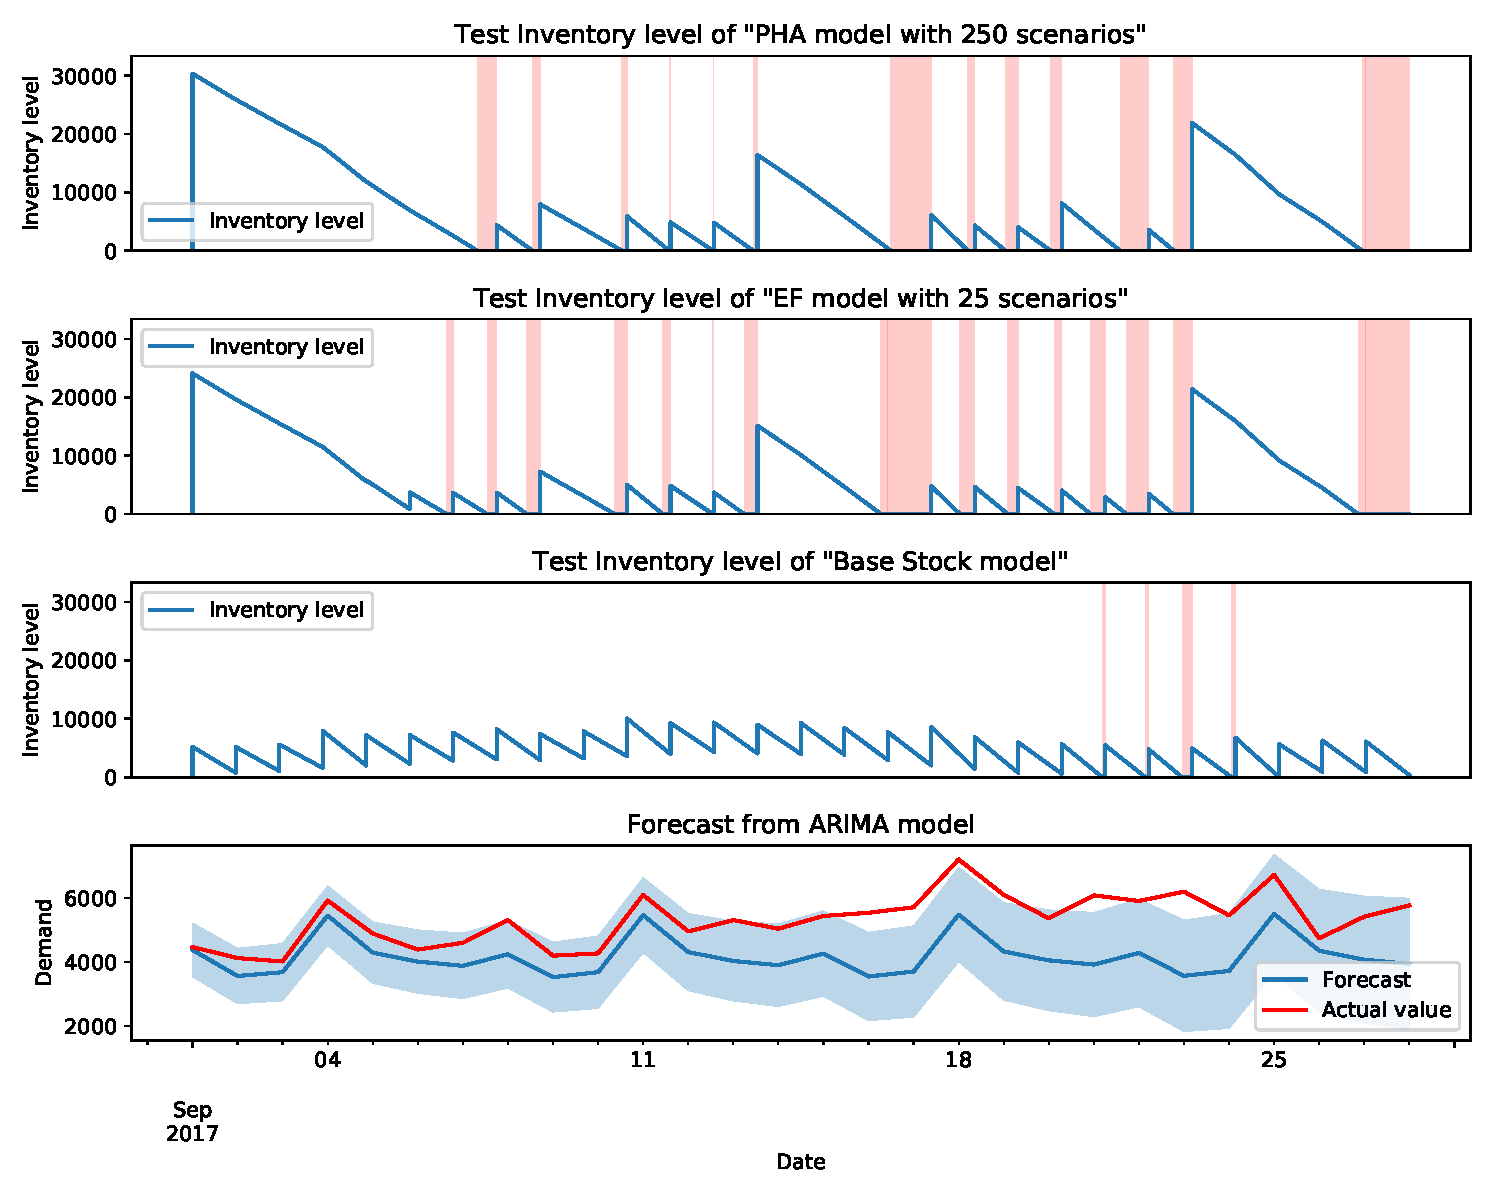
\includegraphics[width=1\linewidth]{figures/cost_sku2_2.pdf}
  \caption[Inventory model simulation visualization for test period 2 of SKU2]{Inventory model simulation visualization for test period 2 of SKU2. The top 3 plots contain inventory level simulations for each model, with periods with shortage highlighted by red rectangles, the bottom plot contains the forecast of ARIMA model with prediction interval in light blue.}
  \label{fig:cost_sku2_p2}
\end{figure}
%%%%%% NEW



\newpage
%%%%%% NEW

The only test case, in which the EF's policy was better than that of PHA  was in case of test case 2 of of SKU5 (visualization in figure \ref{fig:cost_sku5_p2}). However, their policies and estimated costs are almost identical anyway. Both models achieved zero shortage costs, but the PHA model had more excess inventory - its inventory line in the subplot is clearly a little higher. The base stock model had even larger amounts of excess inventory, which resulted in much higher estimated costs.

\begin{figure}
  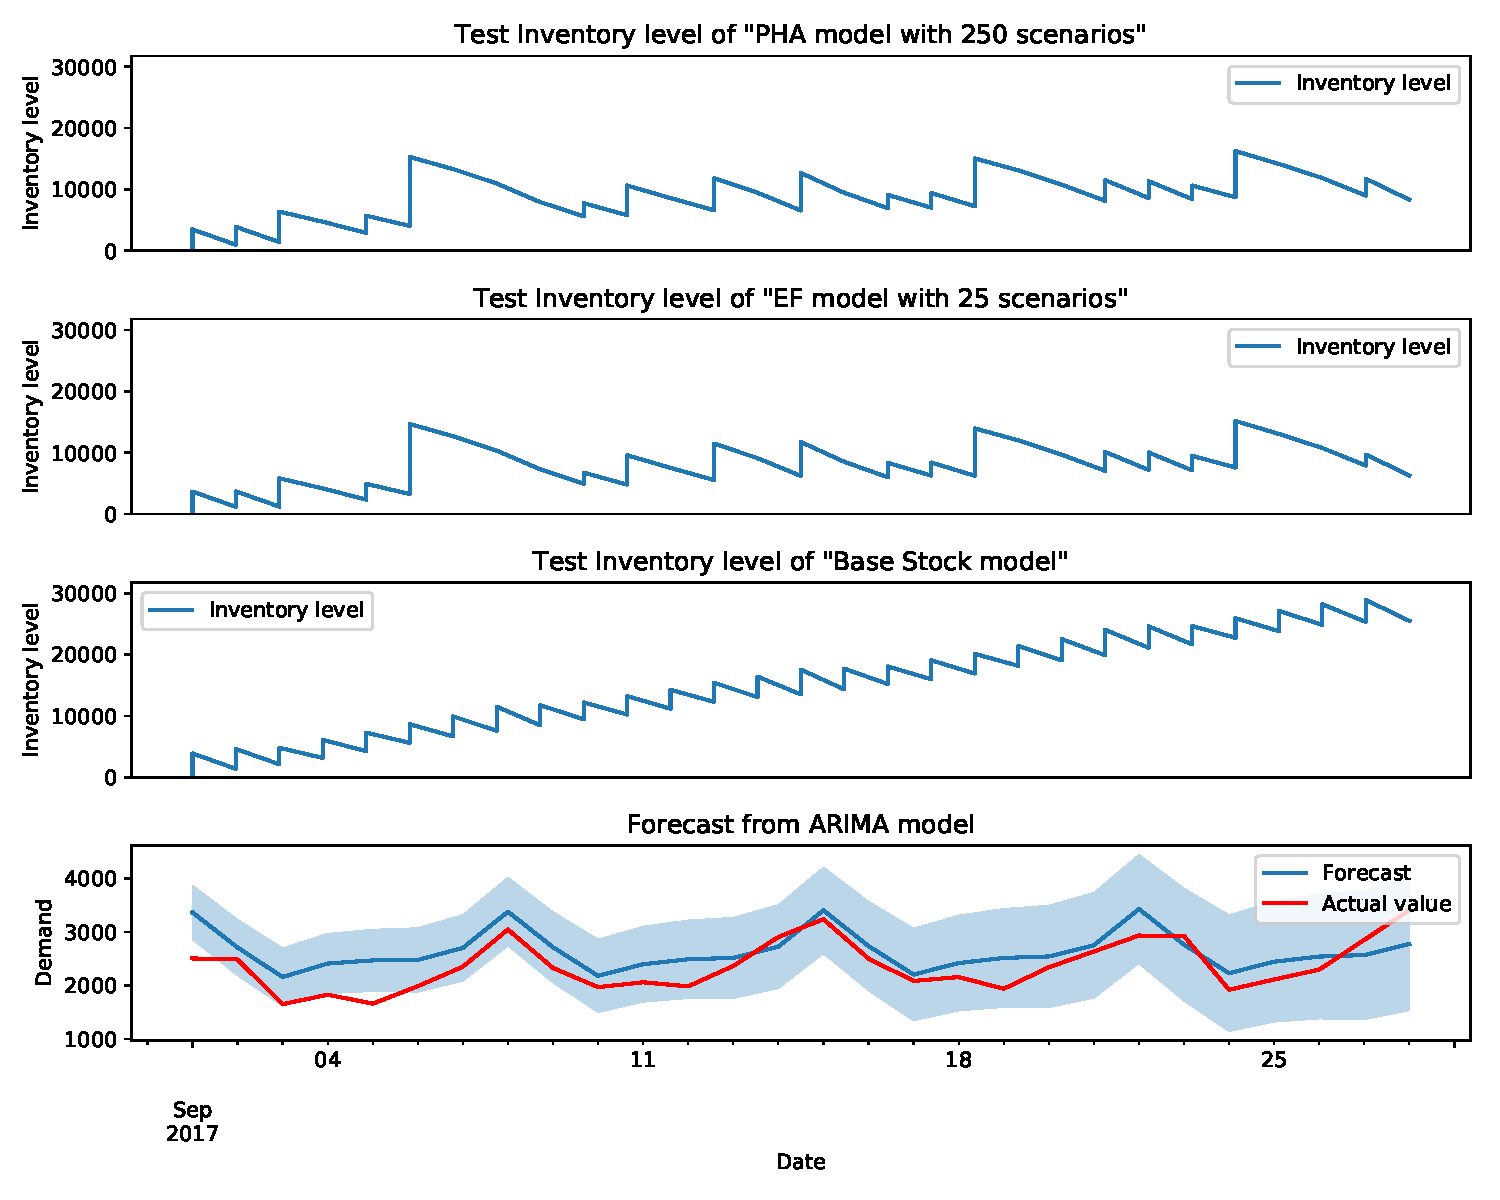
\includegraphics[width=1\linewidth]{figures/cost_sku5_2.pdf}
  \caption[Inventory model simulation visualization for test period 2 of SKU5]{Inventory model simulation visualization for test period 2 of SKU5. The top 3 plots contain inventory level simulations for each model, with periods with shortage highlighted by red rectangles, the bottom plot contains the forecast of ARIMA model with prediction interval in light blue.}
  \label{fig:cost_sku5_p2}
\end{figure}
%%%%%% NEW

\newpage

\begin{table} \catcode`\-=12
\centering
\begin{tabular}{|c|c|c|c|c|c|}
\hline
\multicolumn{3}{|c|}{} &\multicolumn{3}{|c|}{Estimated shortage costs} \\ \hline
\multicolumn{2}{|c|}{}& MAPE &  PHA & EF & Base Stock \\ \hline
\multirow{ 3}{*}{SKU1}& Period 1 & 8.54 & $2.0\cdot 10^4 $ & $7.9\cdot 10^4 $ & 0\\  \cline{2-6}
& Period 2 & 10.17 & $4.6\cdot 10^4 $ & $1.2\cdot 10^5 $ & 0\\  \cline{2-6}
& Period 3 & 10.91 & $9.5\cdot 10^4 $ & $1.5\cdot 10^5 *$ & 0\\ \hline 
\multirow{ 3}{*}{SKU2}& Period 1 & 10.96 & $3.1\cdot 10^4 $ & $8.6\cdot 10^4 *$ & 0\\  \cline{2-6}
& Period 2 & 20.67 & $2.4\cdot 10^5 $ & $3.0\cdot 10^5 *$ & $2.4\cdot 10^4 $\\  \cline{2-6}
& Period 3 & 23.08 & $7.8\cdot 10^3 $ & $10.0\cdot 10^3 *$ & 0\\ \hline 
\multirow{ 3}{*}{SKU3}& Period 1 & 7.23 & $7.3\cdot 10^4 $ & $1.0\cdot 10^5 *$ & 0\\  \cline{2-6}
& Period 2 & 13.10 & $2.5\cdot 10^5 $ & $3.0\cdot 10^5 *$ & 0\\  \cline{2-6}
& Period 3 & 8.66 & $1.6\cdot 10^5 $ & $2.1\cdot 10^5 *$ & 0\\ \hline 
\multirow{ 3}{*}{SKU4}& Period 1 & 10.68 & $1.6\cdot 10^5 $ & $1.8\cdot 10^5 $ & 0\\  \cline{2-6}
& Period 2 & 11.89 & $2.1\cdot 10^5 $ & $2.3\cdot 10^5 $ & 0\\  \cline{2-6}
& Period 3 & 11.28 & $2.7\cdot 10^5 $ & $2.9\cdot 10^5 $ & $1.1\cdot 10^4 $\\ \hline 
\multirow{ 3}{*}{SKU5}& Period 1 & 7.68 & $6.0\cdot 10^3 $ & $5.4\cdot 10^4 $ & 0\\  \cline{2-6}
& Period 2 & 16.25 & 0 & 0 & 0\\  \cline{2-6}
& Period 3 & 8.32 & $6.3\cdot 10^4 $ & $1.3\cdot 10^5 $ & 0\\ \hline 
 \multicolumn{3}{|r|}{Sum }& $1.6\cdot 10^6$ & $2.2\cdot 10^6$ & $3.5\cdot 10^4$\\ \hline 
\end{tabular}
\caption{Estimated shortage costs evaluation}
\label{tbl:shortage_costs}
\end{table}
\subsubsection{Shortage costs evaluation}
We have already provided commentary on the overall performance of the models including shortage costs. Nonetheless the value of shortage costs is not just monetary, as it can cause customer dissatisfaction, so we provide another look at the models, this time with focus on shortage costs.  

Table \ref{tbl:shortage_costs} contains the estimated shortage costs obtained from the inventory simulations. It can be seen that the Base Stock model has the smallest shortage costs overall , which is as expected, because low shortage of goods is the only objective of the model. 
If we look at the columns with results of the PHA and EF models, we can see that the PHA model achieved smaller shortage costs. Therefore we can state, that it has the potential to cause smaller dissatisfaction than the EF model.

\newpage




\subsection{Running time evaluation}
Until now, we have focused on the estimated costs of the generated policies. However another important aspect is the running time of the models, as an inventory might contain thousand of products. Note that we have set a time limit of 1200 seconds for the inventory policy generation, which stopped the Extensive form model before completely finishing in 7 cases. We also won't discuss the running time of the Base Stock model, as it provided the results in an instant in all cases.

As we can see in table \ref{tbl:running_time}, the PHA model was significantly faster than EF in 13 of 15 cases. Its longest test case running time was 669 seconds, however as the algorithm can easily be parallelized, this could be dramatically improved. Even if the running times of EF model were on average significantly longer, it did not provide better results than PHA, except of one test case. The worse time effectiveness of EF meant it had to use smaller count of demand scenarios, and in 7 test cases the EF did not even finish in the time limit anyway.

If we consider that a single powerful machine could theoretically run the EF algorithm for 8 or 16 products at once, an ordering policy for inventory of 1000 products could be generated in roughly 10 hours. With the PHA algorithm, it could finish in 5 hours or even less. Or we could feed even higher count of scenarios in the PHA model, which could further improve its results.




\begin{table} \catcode`\-=12
\centering
\begin{tabular}{|c|c|c|c|c||}
\hline
\multicolumn{2}{|c|}{} &\multicolumn{3}{|c|}{Running time [s]} \\ \hline
\multicolumn{2}{|c|}{} &  PHA & EF & Base Stock \\ \hline
\multirow{ 3}{*}{SKU1}& Period 1  & $256$ & $335$ & $0$\\  \cline{2-5}
& Period 2  & $287$ & $283$ & $0$\\  \cline{2-5}
& Period 3  & $210$ & $1290$ & $0$\\ \hline 
\multirow{ 3}{*}{SKU2}& Period 1  & $332$ & $1200$ & $0$\\  \cline{2-5}
& Period 2  & $258$ & $1201$ & $0$\\  \cline{2-5}
& Period 3  & $284$ & $1200$ & $0$\\ \hline 
\multirow{ 3}{*}{SKU3}& Period 1  & $652$ & $1200$ & $0$\\  \cline{2-5}
& Period 2  & $602$ & $1201$ & $0$\\  \cline{2-5}
& Period 3  & $669$ & $1201$ & $0$\\ \hline 
\multirow{ 3}{*}{SKU4}& Period 1  & $240$ & $978$ & $0$\\  \cline{2-5}
& Period 2  & $506$ & $493$ & $0$\\  \cline{2-5}
& Period 3  & $500$ & $900$ & $0$\\ \hline 
\multirow{ 3}{*}{SKU5}& Period 1  & $161$ & $534$ & $0$\\  \cline{2-5}
& Period 2  & $165$ & $386$ & $0$\\  \cline{2-5}
& Period 3  & $168$ & $614$ & $0$\\ \hline 

\end{tabular}
\caption{Model running time evaluation}
\label{tbl:running_time}
\end{table}
\newpage


\subsubsection{Inventory control evaluation conclusion}
In this subsection we have evaluated three inventory models, first model was the extensive form of our proposed extension of Newsvendor model, which worked with 25 demand realization scenarios in each test case, the second one was the a decomposed version of the previous model, which used the Progressive Hedging Algorithm and 250 demand scenarios. The last model was the simple Base Stock model.

Across 3 testing periods for 5 SKUs, forming 15 possibly real world test cases, the best on average model was the PHA base model, as it generated inventory policies with the smallest cost. Its extensive form provided worse results, which were obtained in significantly longer running times.

The Base Stock model was the worst performing one, as it does not consider price changes and also due to the relatively accurate forecasts, its safety inventory level was not needed in most cases.

\subsection{Evaluation conclusion}
In this section, we have evaluated both the demand forecasting models and the inventory control models. For the purposes of evaluation, we have extracted 15 possibly real world test cases from the data provided by the supervisor. 

Both the exponential smoothing and ARIMA forecasting models showed reasonable forecasting performance given the random nature of the 
testing data. However, during our in depth analysis we have found out that the ``fitting'' procedure of both models could be further improved. Possible future work could therefore focus on the fitting phase, or on forecasting with external factors.

In the part dedicated to inventory control, we compared the performance of two version of our extended Newsvendor inventory model. This model has the advantage of large variability due to its
mixed integer linear programming formulation, but solving the program requires large amounts of computation time. Therefore we have compared  the extensive formulation of the model and its approximation form based on Progressive Hedging Algorithm.
The extensive form of the model had to use less demand information in order to be able to finish in reasonable computing time. The approximation form had the advantage of more demand information. 

The PHA model performed significantly better on average than the extensive form, and it required significantly less computation time.
Both models performed better than the the third model - the simplistic Base Stock model.
In future work, we could focus on development of some combination of these models. The decomposition formulation could be used to presolve parts of the problem, until a smaller problem is obtained, which could be later solved in the extensive form.

\newpage
\section{Conclusion}
The task of this thesis was to study the problems of demand prediction and inventory optimization, and to employ this knowledge to create an automated inventory control model. After a thorough analysis we have presented a set of time series forecasting and inventory control approaches, which together form an inventory control pipeline capable of generating possibly optimal goods ordering policies.

The demand prediction part of the thesis contains a survey of time series forecasting problematic and available methods. The prediction part of the inventory control pipeline was then implemented to include an extended exponential smoothing forecasting method and a seasonal ARIMA model. Both methods have proven its worth in many previous research works and results of our evaluation confirm they are suitable for our task as well.


The inventory control part of the thesis consists of an introduction to the inventory control problematic, and contains a review of important concepts of stochastic programming, which are highly useful for inventory models that assume demand uncertainty. We then proceed by creating an extension of the stochastic multi-stage Newsvendor inventory model, that can generate ordering policies for many time periods ahead. This model considers fixed and per unit ordering costs, shortage costs, holding costs and goods durability. All costs can be time-dependent and the model can be possibly extended even further, as it has a flexible mixed integer linear program formulation. We then suggested to solve the problem using the progressive hedging algorithm to improve the model's efficiency and significantly enhance its ability to hedge its inventory policies against more demand outcomes.


We have performed a two stage, in depth evaluation of the proposed methods, using real world data.
In the first stage, which was dedicated to evaluation of the forecasting methods, the seasonal ARIMA model proved its superiority and robustness. Its forecasts were always either the most accurate, or very close to the best forecast, and its performance was the most stable. Its residuals showed that it fitted the provided data well, as its errors showed almost no correlation, and normality. The second stage evaluated the proposed inventory models by estimating costs of their inventory policies and compared the models from the customer satisfaction perspective. We also examined the trade of between solving an exact form of the inventory model with limited amount of demand scenario samples, and solving its approximation with significantly more demand scenarios. The results showed that it is sufficient to use reasonable number of scenarios to achieve efficient inventory control policy, and it is preferable to use the approximation approach. The approximation form provided the best inventory policies due to the significantly larger amount of demand scenarios it could handle, and its running times were much lower than those of the exact form.

\subsection{Future work}
We can name multiple examples of possible improvements and topics for possible future research.  

The demand prediction module's accuracy could be improved by including a forecasting method that uses external factors in addition to the historical time series data, such as SARIMAX. 

It would be interesting to focus on the scenario generation procedure as well. For example we could test other methods of the forecast prediction interval estimation, such as bootstrapping the residuals.

The inventory module could be improved by combining the decomposition approach and the extensive form solution approach. The decomposition model could be used to generate a subset of the inventory decisions, until a problem of manageable size for the extensive form is obtained. The extensive form could then generate optimal decisions for the remaining problem. 

\newpage
\section{Appendix}
\label{sec:appendix}
\begin{table}
  \caption{Demand forecasting evaluation results}
  \label{tbl:dem_bench}
  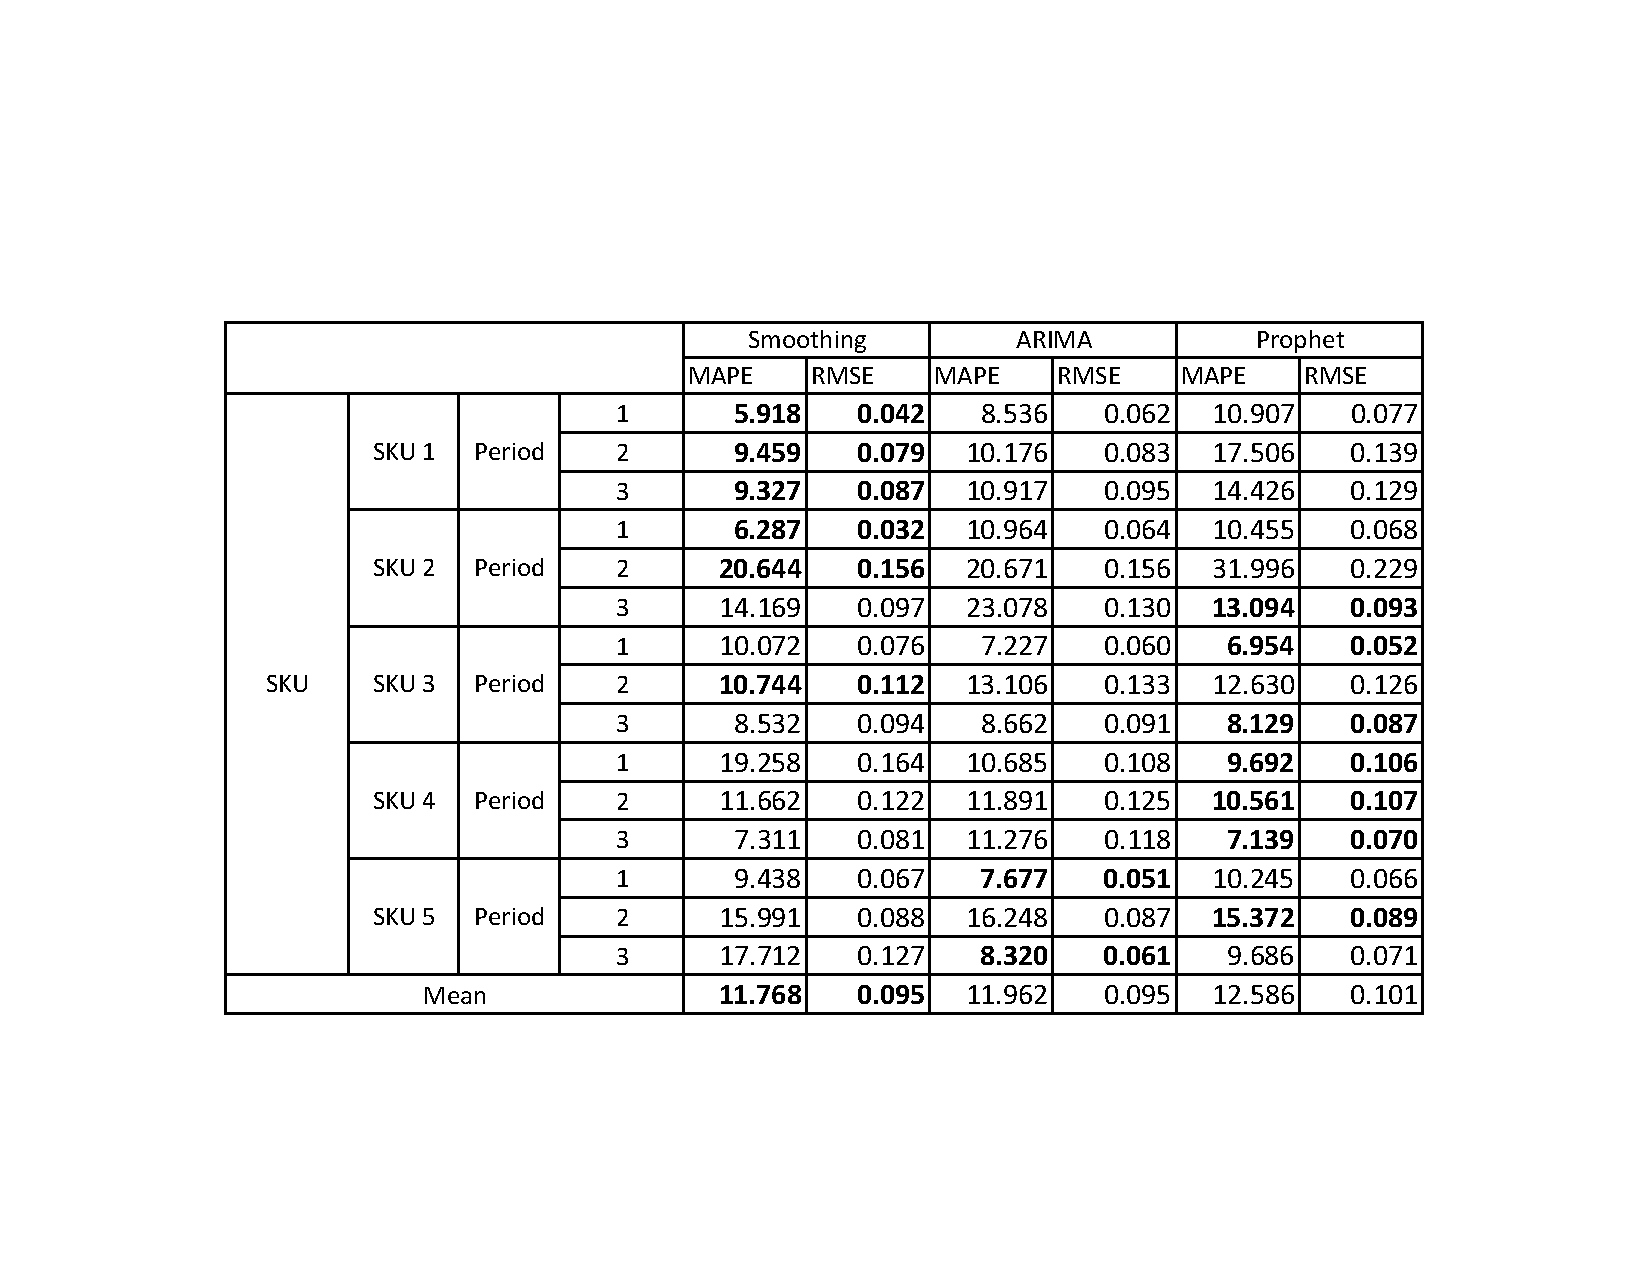
\includegraphics[angle=270,origin=c,width=1.3\textwidth]{figures/experiments1.pdf}
\end{table}

\newpage
\begin{figure}
  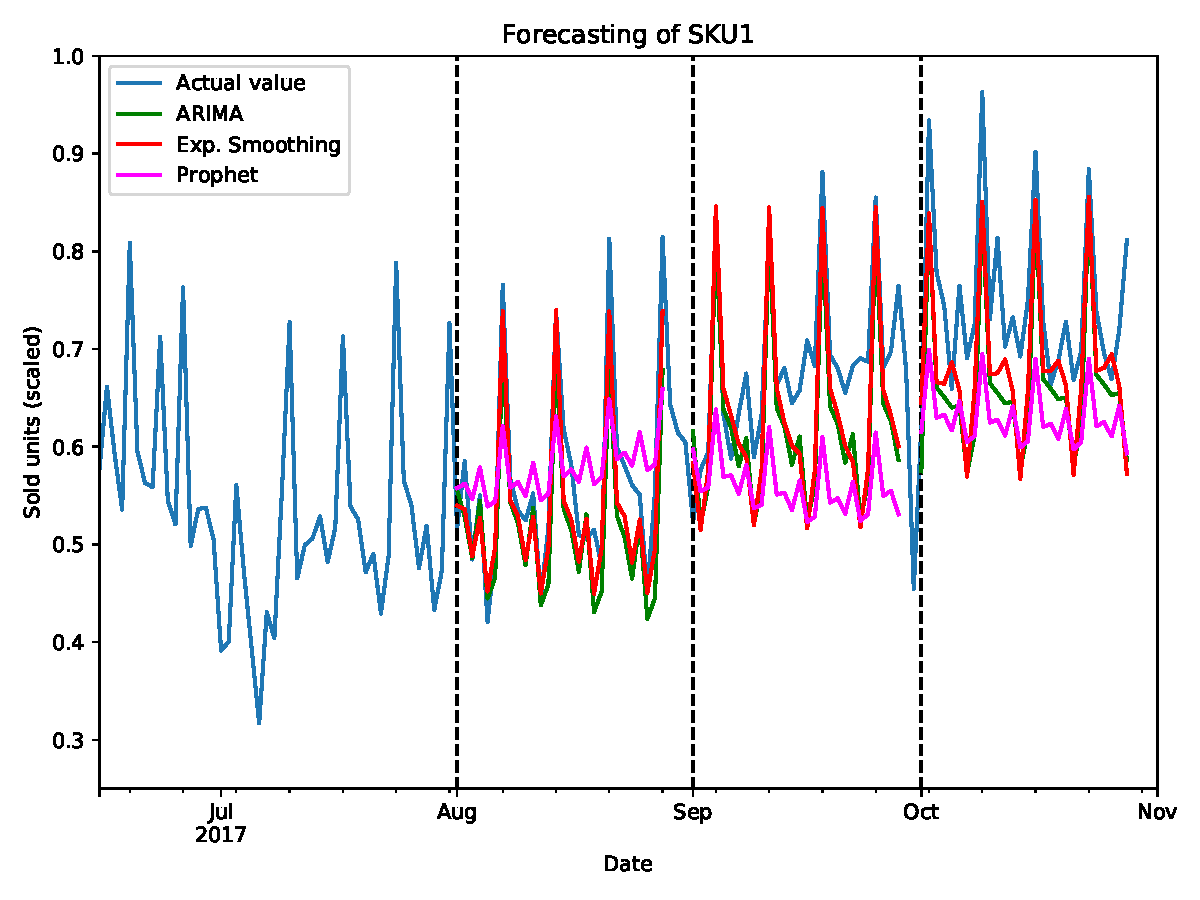
\includegraphics[width=1.2\linewidth]{figures/SKU1_all.pdf}
  \caption{Results of first product class forecasting evaluation}
  \label{fig:sku1_all}
\end{figure}

\begin{figure}
  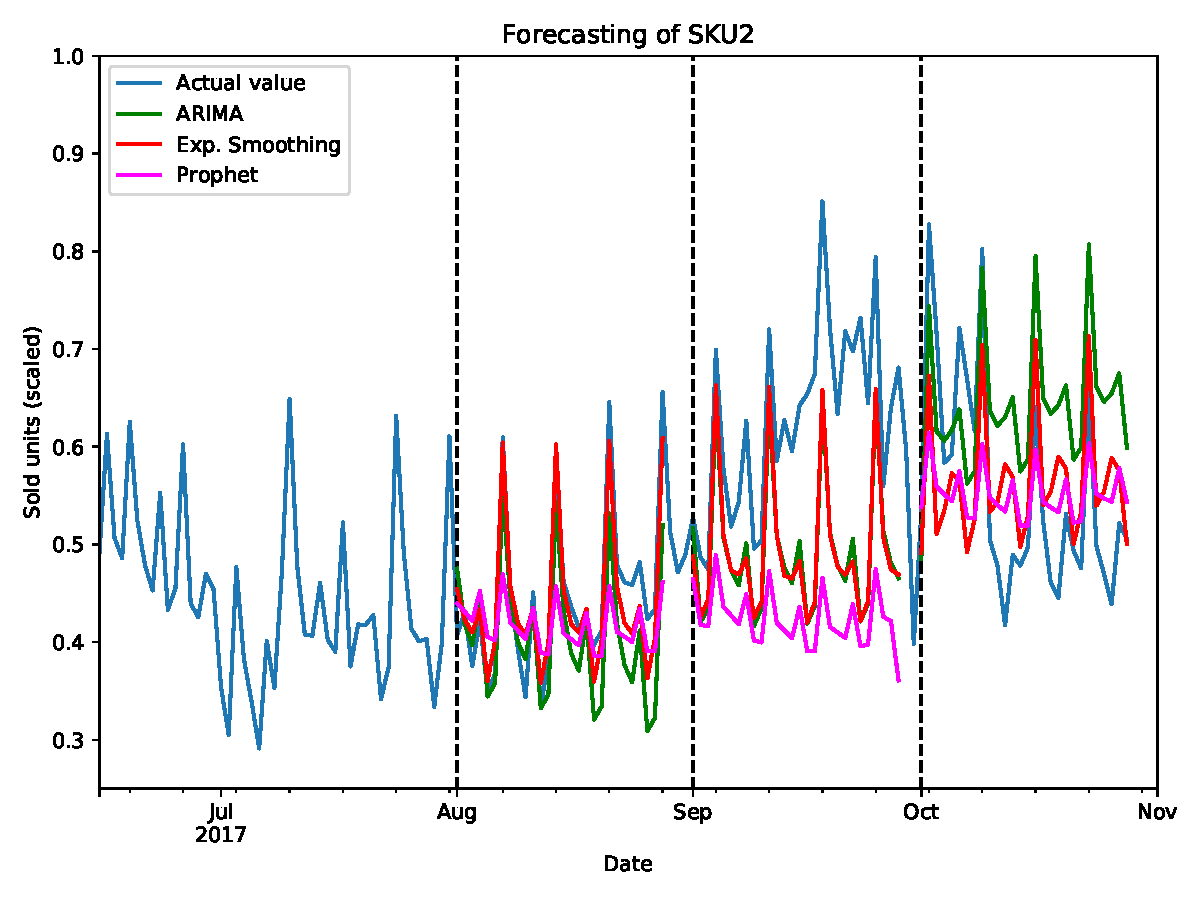
\includegraphics[width=1.2\linewidth]{figures/SKU2_all.pdf}
  \caption{Results of second product class forecasting evaluation}
  \label{fig:sku2_all}
\end{figure}

\begin{figure}
  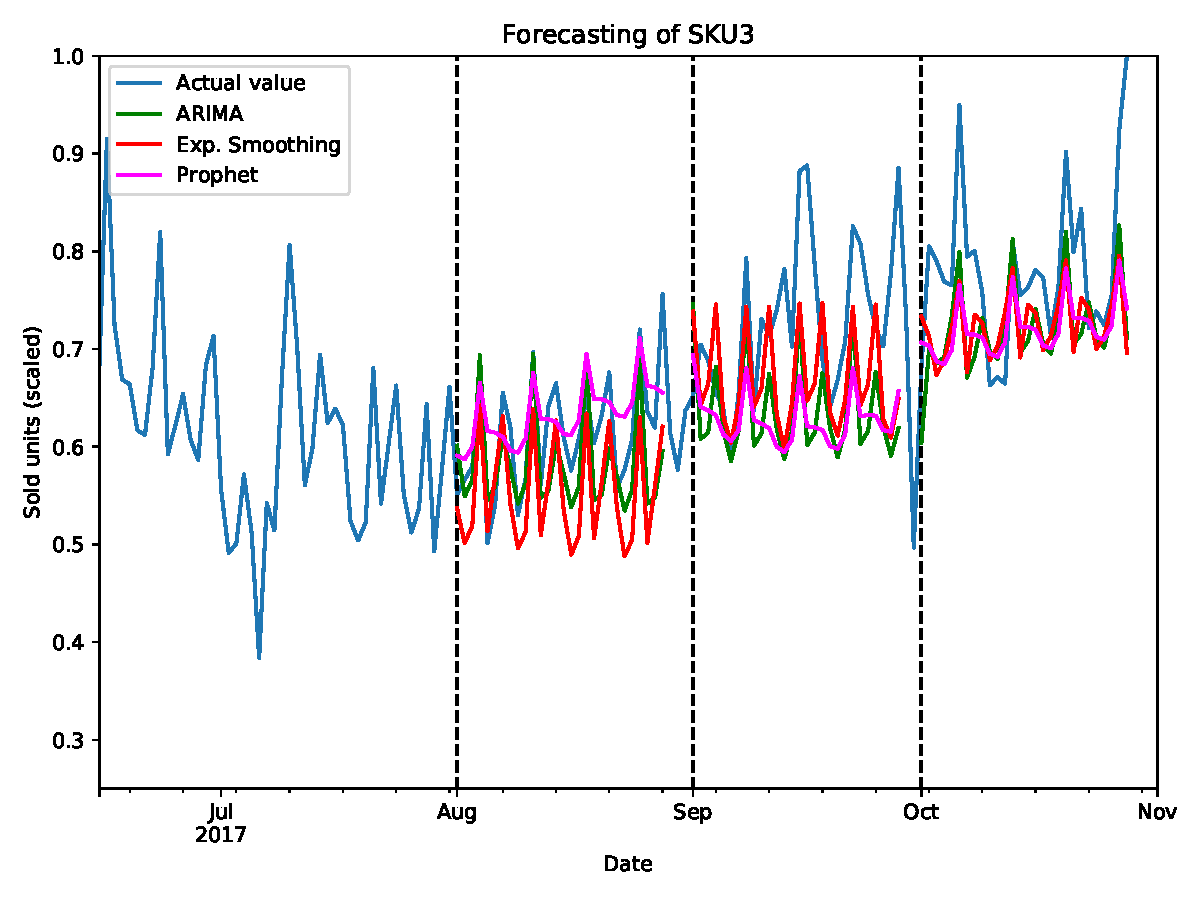
\includegraphics[width=1.2\linewidth]{figures/SKU3_all.pdf}
  \caption{Results of third product class forecasting evaluation}
  \label{fig:sku3_all}
\end{figure}

\begin{figure}
  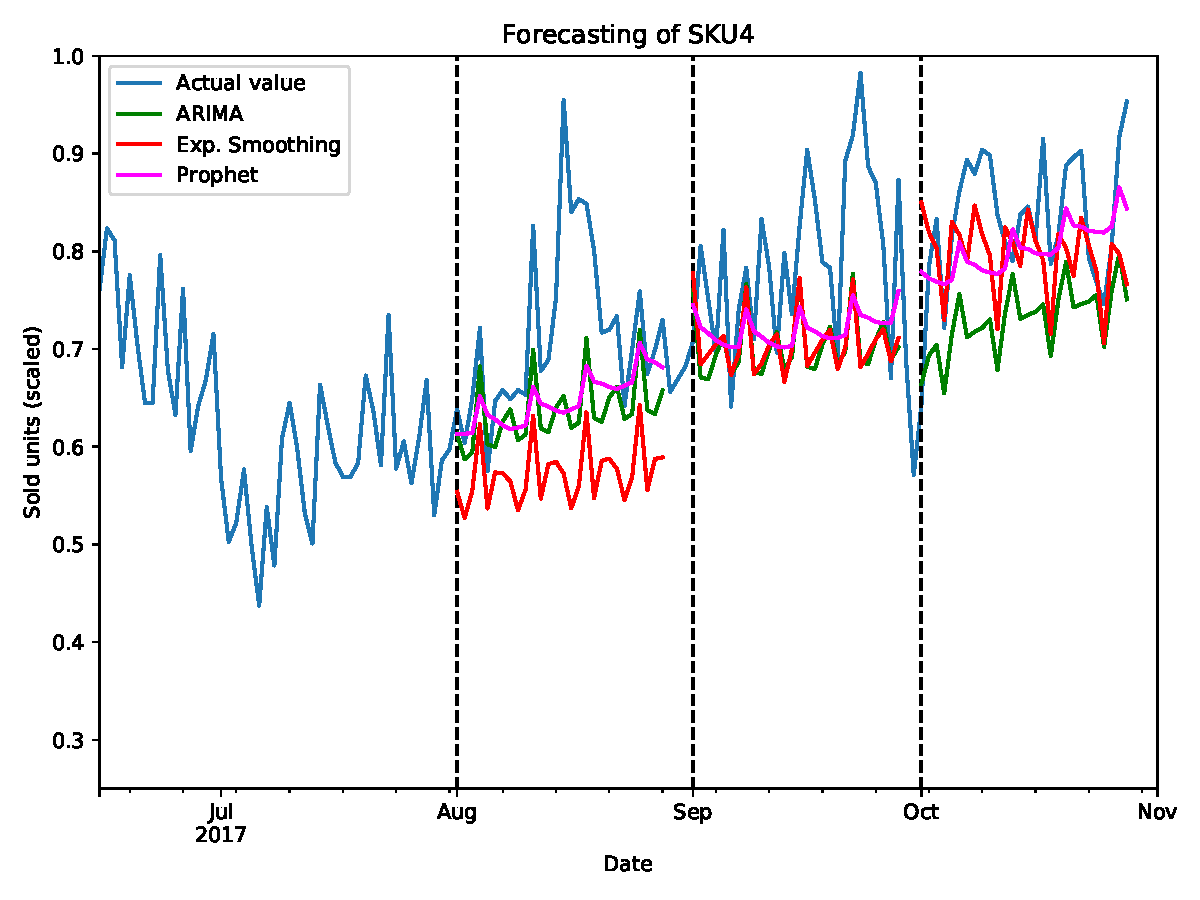
\includegraphics[width=1.2\linewidth]{figures/SKU4_all.pdf}
  \caption{Results of fourth product class forecasting evaluation}
  \label{fig:sku4_all}
\end{figure}

\begin{figure}
  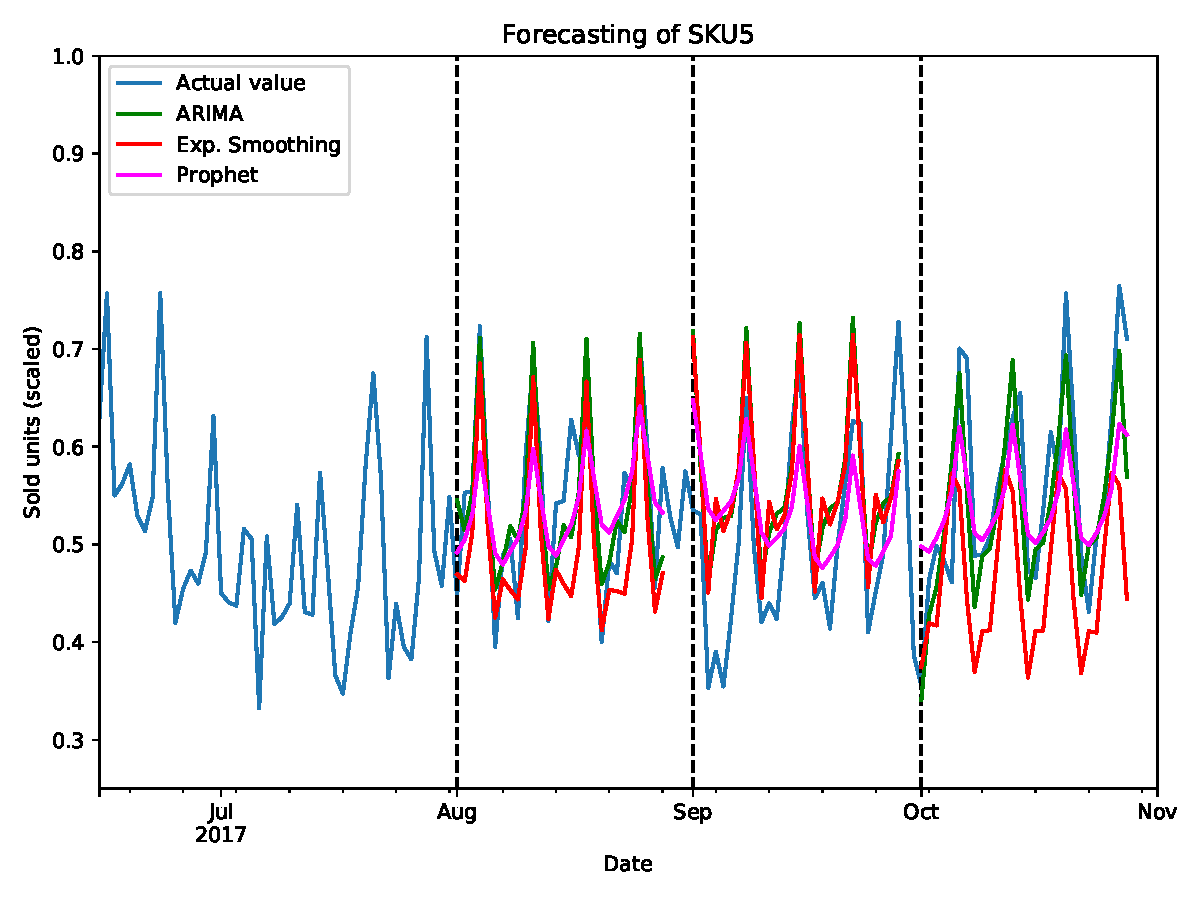
\includegraphics[width=1.2\linewidth]{figures/SKU5_all.pdf}
  \caption{Results of fifth product class forecasting evaluation}
  \label{fig:sku5_all}
\end{figure}


\newpage
\clearpage
\bibliography{file}
\bibliographystyle{unsrt}
\addcontentsline{toc}{section}{~~~References}
\newpage
\listoffigures
\newpage
\listoftables
\end{document}
